% This work is licensed under
% http://creativecommon.org/licenses/by/3.0/
%\documentclass{article}
\documentclass[ebook.tex]{subfiles}
%\usepackage{graphicx}
%\usepackage{latexsym}
%\usepackage{amsmath}
%\usepackage{color}
%\usepackage{url}
%\hyphenation{wrap-around}

%this is a nice-looking bullet list:
%\begin{list}{$\bullet$}{
%                      \setlength{\topsep}{0in}
%                      \setlength{\itemsep}{0in}
%                      \setlength{\parsep}{0in}
%                      \setlength{\leftmargin}{.13in}
%                     }
%\item
%\end{list}

%this is a two-column figure:
%(for a one-column figure, remove *)
%figure must be in ???.pdf
%\begin{figure*}[hbt]
%\begin{center}
%\includegraphics[scale=1.00]{???}
%\end{center}
%\caption{???}
%\label{fig:???}
%\end{figure*}

%this is a two-column, floating table:
%(for a one-column table, remove *)
%(for a non-floating table, remove table environment)
%\begin{table*}
%\begin{tabular}
%\end{tabular}
%\end{table*}

%JEN: for new text added by jen.  can simply remove \textcolor{red} to
%get rid of red color, or remove the \jen{} where it appears in the text.
\newcommand{\jen}[1]{\textcolor{red}{#1}}

\title{The Design Space of Network Mobility}

\author{
Pamela Zave \\
AT\&T Laboratories---Research \\
Florham Park, New Jersey, USA \\
{\tt pamela@research.att.com}
\and
Jennifer Rexford \\
Princeton University \\
Princeton, New Jersey, USA \\
{\tt jrex@cs.princeton.edu}
}

\pagestyle{empty}

\begin{document}
\pagestyle{empty}
\maketitle

\pagestyle{empty}

\begin{abstract}
While the Internet is increasingly mobile, seamless mobility is
difficult to implement at Internet scale.  Over the years, standards
bodies and the research community have introduced a large and
confusing collection of mobility proposals that are difficult to
compare.  In this tutorial, we present these mobility proposals
in a uniform framework, called the geomorphic view of networking.
The geomorphic view shows that there are two distinct patterns
for implementing mobility, each with its own range of 
design choices and cost-benefit trade-offs.
We use these patterns to classify and explain
a representative sample of mobility
mechanisms, abstractly yet precisely.
The patterns also serve as a basis for evaluating properties of
these mechanisms such as resource costs and scalability,
and for considering composition of mobility mechanisms.
\end{abstract}

% This work is licensed under
% http://creativecommon.org/licenses/by/3.0/
\section{Introduction}
\label{sec:sec1}

The Internet is increasingly mobile.  
Users access Internet services from mobile devices that move from one
wireless access point to another, or switch between WiFi and cellular 
network connectivity.  
Ubiquitous computing relies on sensors and actuators attached to vehicles,
portable objects, and animals as well as people.
Applications 
provide customers with application-level identities that can be
used to reach them at whichever device they are currently using.
Increasingly, software runs on virtual machines that can migrate from one
physical server, or even one data center, to another.

We define network
mobility as the capability that allows a communicating entity
to continue to communicate over a network, despite the fact that its
location at (or binding to) a lower-level communicating entity is changing.
Further, we focus on so-called ``seamless'' mobility, in which the
high-level entity's communication channels are preserved throughout
the change.

It is important to note that this definition applies at all conceptual
levels.
A person can have an identifier as a communicating entity, and can be
mobile by moving from one networked device to another.
A device such as a
cellphone can have an identifier, and can be mobile by moving from one
network attachment point to another.
An interface on a device, such as an Ethernet interface, can have an
identifier and be mobile by moving within or between local area networks.

In recent years, many mechanisms have emerged for supporting 
mobility.
A recent survey~\cite{rfc6301} cites 22 Internet protocols dating from 1991
to 2009, including most prominently Mobile IPv4, Mobile IPv6,
MSM-IP, HIP, MOBIKE,
Cellular IP, HAWAII,
ILNP, and LISP Mobile Node.
In other contexts mobility is supported by:
\begin{itemize}
\item
Ethernet LANs and VLANs, which allow an interface to retain its IP address 
as the host moves within the LAN;

\item 
the scalable ``flat'' routing architectures 
SEATTLE \cite{seattle}, PortLand~\cite{portland},
VL2~\cite{vl2}, NVP~\cite{nvp}, and
Rbridges/TRILL~\cite{rbridges,rfc5556}
that also naturally support routing to an interface that
retains its addresses as the host move;

\item
injecting the IP address of a mobile machine into existing routing protocols
such as OSPF and BGP~\cite{connexion,smog};

\item
the General Packet Radio Service (GPRS) Tunneling Protocol (GTP),
which supports mobility in most cellular networks;

\item
other research proposals including
TCP Migrate \cite{tcp-migrate}, Serval \cite{serval}, 
and the Internet Indirection Infrastructure~\cite{i3};

\item
application-level protocols such as 
the Session Initiation Protocol (SIP)~\cite{mobilesip}.
\end{itemize}

\noindent
Each well-known proposal tends to spawn a family of variants, so
the total number is probably in the hundreds and growing.

These various mechanisms operate at different levels, and make
different assumptions about naming, routing, session
protocols, scale, security, and the cooperation of
remote endpoints or multiple administrative domains.  
Because the
community lacks a common framework for describing and comparing
mobility mechanisms, their relationships are poorly understood.
Comparisons tend to be based on superficial characteristics rather
than inherent ones.  
Quantitative comparison must be based on
labor-intensive prototyping and measurement or simulation.

This book chapter has two goals:
\begin{itemize}
\item
To describe and compare existing proposals for implementing mobility.
\item
To map out a design space in which
new mobility mechanisms can be discovered,
evaluated, and exploited.
\end{itemize}

\noindent
To achieve these goals,
we explain mobility in a new way.
We begin by defining a common framework for describing network
architectures.
This framework is
called the {\it geomorphic view} of networking, and is
introduced in
Section~\ref{sec:sec2}.

The geomorphic view has been developed to be simple, modular,
comprehensive, and formalizable.
It supports the first goal by providing a precise, unique description
of each mobility mechanism
that omits inessential detail while exposing subtle differences
and important engineering trade-offs.

The common framework supports the second goal in several ways.
It allows us to generalize over the implementations of mobility,
showing that they are all instances of two major patterns.
It also allows us to understand how 
different instances of the mobility patterns at different places in a
network
architecture can be composed, generating a potentially large design
space to be explored.

Section~\ref{sec:sec3} of this chapter introduces the two major
patterns---\emph{dynamic-routing mobility}
and \emph{session-location mobility}---for implementing mobility.
If they are both implemented within an IP layer, the difference centers
on whether a mobile machine
retains its IP address when
it moves, or changes its IP address and updates its correspondents.
Each pattern has a completely different set of subsidiary design
decisions and resource costs.

The next sections 
use the patterns to describe and compare many of the most
important proposals for mobility.  
Sections~\ref{sec:sec4} and
\ref{sec:sec5} compare different ways to implement
dynamic-routing mobility,
with a non-hierarchical name space ({\it e.g.,}
MAC addresses in a local area
network) or a hierarchical name
space ({\it e.g.,} IP addresses in the wide
area), respectively.  
Section~\ref{sec:sec6} compares four prominent protocols for
session-location mobility at different stages in the IETF
standardization process.

Section~\ref{sec:sec7} of the chapter turns to
a more systematic exploration of the
design space, first showing that there may be some freedom concerning
where in an architecture a particular kind of mobility is handled.
The section also discusses composition of mobility
mechanisms.
As an example, we illustrate how Mobile IPv6 is a
composition of both the dynamic-routing mobility and session-location
mobility design patterns.

Finally, Section~\ref{sec:sec8} surveys several topics closely
related to mobility, including multihoming, anycast services, site
mobility, incremental deployment of mobility protocols, and security
issues for mobility.  
The chapter ends with a brief
conclusion outlining several more advanced areas of study.


% This work is licensed under
% http://creativecommon.org/licenses/by/3.0/
\section{The geomorphic view of networking}
\label{sec:sec2}

The geomorphic
view of networking was originally inspired by the work of Day \cite{pna},
although we have made many changes and additions in both content and
presentation.
In this common framework for describing networks,
the module is a
{\it layer}, and a network architecture is a hierarchy of layers.

\subsection{Comparison with the Internet and OSI models}
Layers may seem familiar and obvious because both the classic Internet
architecture \cite{philo} and the
OSI reference model \cite{OSI}
also describe network architecture as a hierarchy of layers.
However,
our concept of a layer is very different.
As a preview of this section, our layer hierarchies differ from these
earlier ones in at least four ways:
\begin{itemize}
\item
The classic Internet architecture and the OSI reference model both have
a fixed number of levels.
In a geomorphic layer hierarchy, there can be any number of levels.
\item
In the earlier models, there is only one layer on each level, so there
is no distinction between layer and level.
In a geomorphic hierarchy, there can be multiple layers on the same
level.
\item
In the earlier models, each layer has a specific function that is
distinct from the functions of other layers.
In the geomorphic view
each layer is a microcosm of networking, containing all of the basic
components and functions in some form.
In different layer instances there are different versions of these
basic ingredients, used at
different levels, with different scopes, and for
different purposes.
\item
Most people interpret the earlier models as describing the data
plane of networking only.
The control plane is seen as separate and not modularized in the
same way.
In the geomorphic view, each layer---being a microcosm of
networking---has a data plane and a control plane.
Layers decompose both planes into modules.
\end{itemize}
Figure~\ref{fig:geoname} illustrates these differences, and also
shows how the ``geomorphic'' view got its name.
The complex arrangement of layers, with overlapping, abutting, and
bulging shapes, can resemble the complex arrangement of layers in the
earth's crust.

\begin{figure}
\centering
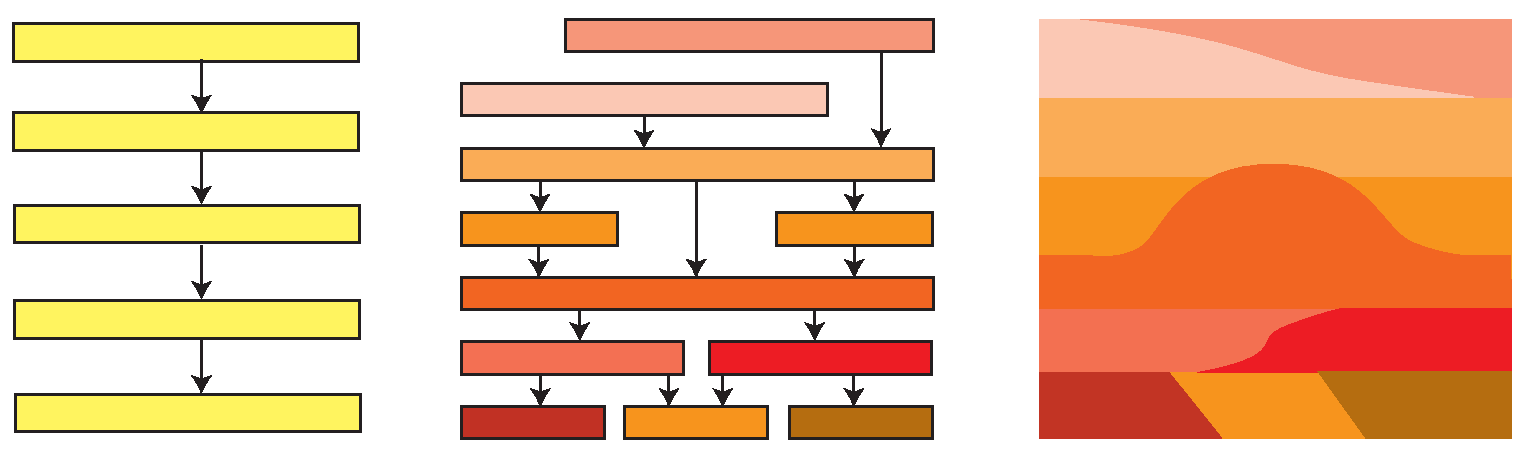
\includegraphics[scale=0.45]{figures/geoname.pdf}
\caption{Arrangement of layers in the classic Internet architecture
(left), the geomorphic view (middle), and the earth's crust (right).}
\label{fig:geoname}
\end{figure}

\subsection{Components of a layer}
\label{sec:layercomponents}

A layer has {\it members}, each of which has a unique and persistent
{\it name} within the layer.
For example, Figure~\ref{fig:layer} is a snapshot of a layer with five
members, each having a capital letter as a name.
In general a member is a concurrent process, {\it i.e.,} a locus
of state and control with the potential for autonomous action.

The members of a layer communicate with each other through {\it links},
shown by lines in Figure~\ref{fig:layer}.
A link is a communication channel.

\begin{figure}
\centering
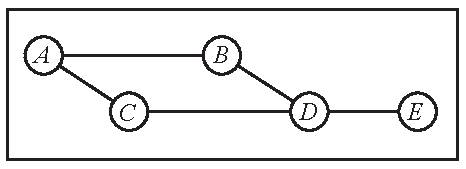
\includegraphics[scale=0.80]{figures/littlelayer.pdf}
\caption{Members and links of a layer.}
\label{fig:layer}
\end{figure}

One of the two primary functions of a layer is to enable members to send
messages to each other.
This function is accomplished by a {\it forwarding protocol},
which runs in all members and has operations for sending and
receiving messages over the links.

In general, a layer does not have a link between each pair of members.
Such a layer needs {\it routes}
indicating how one member can reach another through links and
intermediate members.
For example, ({\it A, B, D, E} ) is a route from {\it A} to {\it E}.
If {\it B} receives a message that is destined
for {\it E}, its forwarding protocol uses the route information
to forward the message to {\it D} on its way to {\it E}.

The {\it routes} are shared state of the layer, and a simple 
geomorphic description need say no more about them. 
To provide more realistic detail, in a real layer the {\it routes}
information is often distributed over forwarding tables found in
the individual members.

The other primary function of a layer is to implement enriched
end-to-end
communication services on top of its bare message transmission.
This function is carried out by a {\it session protocol}.
The forwarding protocol can be unreliable, especially if links are
dynamic and the current routes are obsolete.
A session protocol can provide services including reliability,
FIFO delivery,
and quality-of-service guarantees.
Figure~\ref{fig:impl} shows a session between endpoints {\it a}
and {\it e} of the lower layer.

A {\it channel} is an instance of a communication
service.
Both links and sessions are channels.
A layer can implement its own links internally, and a
layer can implement its sessions for the benefit of its own
members.

Most commonly, however, a link in one layer is
implemented by a session in another layer,
as shown in Figure~\ref{fig:impl}, placing the other
layer lower in the {\it ``uses'' hierarchy}.
If an underlay (lower layer) is implementing a link for an overlay
(higher layer), then the basic attributes of the channel must be
stored in the states of both layers.
In the overlay, the channel object is one of its {\it links}.
In the underlay, the channel object is one of its {\it sessions}.
There must be two names for the sets of channels of interest to a layer,
because a typical layer both uses {\it links} and 
implements {\it sessions}.

For a link in an overlay to be implemented by a session in an underlay,
both endpoint {\it machines} must have members in both layers,
as shown in Figure~\ref{fig:impl}.
The boundary of a
{\it machine} is the boundary of an operating system that provides fast,
reliable communication between members of different layers on the machine.
This fast, reliable operating-system
communication is the foundation on which networked
communication is built.\footnote{Although layer members have been
described as concurrent processes, they are not usually ``processes''
as defined by the operating system; processes in an operating system
have many more properties and associations than layer members do.  
A virtual machine can be regarded as a {\it machine}, in which case
communication through the hypervisor and soft switch of the physical
machine is regarded as networked communication.}

\begin{figure}
\centering
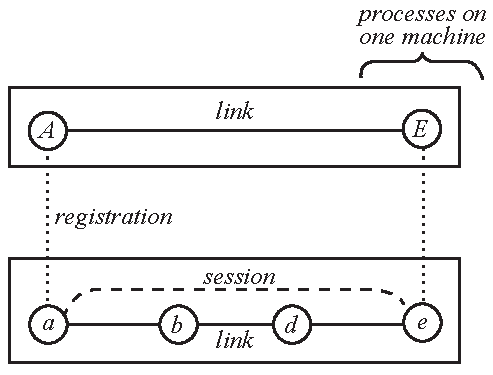
\includegraphics[scale=0.80]{figures/impl.pdf}
\caption{Implementation of a link in an overlay by a session in an
underlay.}
\label{fig:impl}
\end{figure}

The relation between an overlay member and an underlay member on the
same machine is called {\it registration}.
Registrations must be stored in the state of both layers.
In the overlay a registration is recorded as an {\it attachment}, 
which says that the overlay member is attached to the network through
a particular lower layer.
In the underlay a registration is recorded as a
{\it location}, 
which says that a particular member of a particular overlay is attached to
the network at a particular member (its location) of this layer.

The session protocol creates and maintains {\it sessions} data in its
layer, and uses {\it locations} data.
For example, in Figure~\ref{fig:impl}, {\it A} sent a request to {\it a}
for a session with {\it E}.
To create this session, {\it a} learned from its layer's {\it locations}
that {\it E} is currently located at {\it e}.
Messages sent from {\it A} to {\it E} through the link in the overlay
travel through {\it a, b, d,} and {\it e}; the first and last steps
uses operating-system communication, while the middle three steps use
networked communication.

All the major components of a layer are shown in
Figure~\ref{fig:table}.
The forwarding and session protocols perform the two primary functions
of the layer.
These protocols and their operations are collectively known as the
``data plane'' of the layer.
The network's data plane also includes the inter-layer interfaces
through which the endpoints of an implemented link transfer messages to 
and from the
implementing session.

There are six major state components, all of which 
can be dynamic.
We have seen that the session protocol creates and maintains
{\it sessions};
the other five are created and maintained by their own maintenance
algorithms.
The state and algorithms are collectively known as the ``control plane''
of the layer.
Note that the network's control plane also includes the inter-layer
interfaces through which the control algorithms communicate.

\begin{figure}
\centering
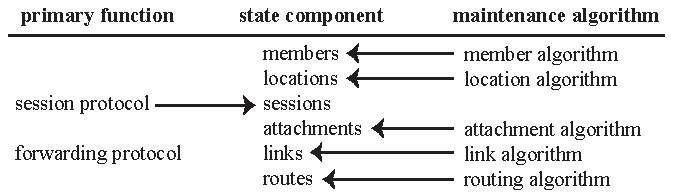
\includegraphics[scale=1.00]{figures/table.pdf}
\caption{Major components of a layer.  Arrows show which protocol
or algorithm writes a state component.}
\label{fig:table}
\end{figure}

\subsection{Layers within a network architecture}

Figure~\ref{fig:scope} shows a geomorphic view of the classic
Internet architecture.
The {\it scope} of a layer is its set of potential members.
For example, 
at the top level of the hierarchy, there are two application layers.
The scope of each layer is the set of potential processes running
software for that application.
These layers are pictured as overlapping because the horizontal
dimension is an approximation of geographical space, and both
applications can have members world-wide.
In particular, the registration lines in the diagram show that each
application has a member on one particular machine.

\begin{figure}
\centering
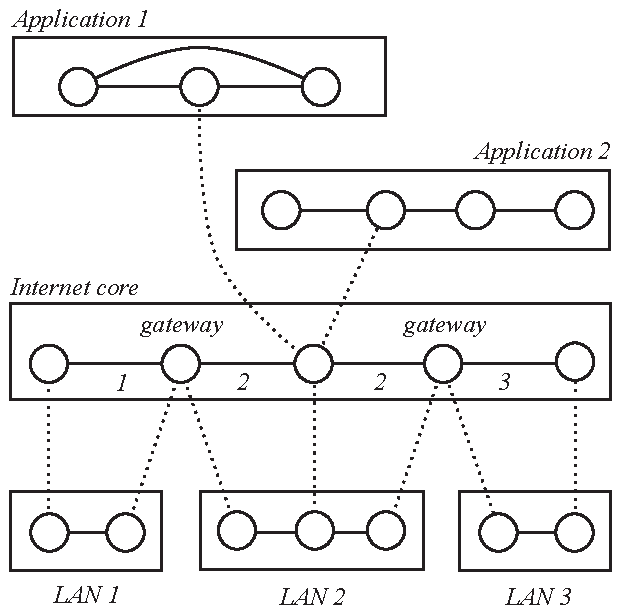
\includegraphics[scale=0.80]{figures/newip.pdf}
\caption{Geomorphic view of the classic Internet architecture.
Internet links are labeled with the LAN that implements them.}
\label{fig:scope}
\end{figure}

In the middle level of the hierarchy there is a single layer called
the ``Internet core.''
Its members are the IP interfaces of networked machines.
In this layer, IP (the ``network layer'' of the classic Internet
architecture) is the forwarding protocol, and TCP and UDP
(the ``transport layer'' of the classic Internet architecture)
are variants of the session protocol.

At the bottom level of the hierarchy there are local area networks
(LANs) with local scopes.
Each LAN member is an interface appropriate to the type of LAN.
For example, for an Ethernet LAN, the members are the Ethernet interfaces
of machines.
Figure~\ref{fig:scope} illustrates the point, made in the preview
of this section, that in the geomorphic view there can be multiple layers
at one level of the ``uses'' hierarchy.

Note that every member of the Internet core is attached to a member
of a layer at the bottom level.
Note especially that for two members of the Internet core layer to
be linked, both of those members must be attached to the same layer
at a lower level, so that the lower layer can implement the link.
This observation is important for understanding mobility.
A gateway in the Internet core layer is attached to multiple LANs, 
so it can forward messages from one LAN to another.

Because layers instantiated at different levels have different purposes,
they have different versions of the common components enumerated in
Figure~\ref{fig:table}.
For one
example, the best-known routing algorithms are found in the Internet
core, where their purpose is reachability.
Now consider a middleware layer, above the Internet core,
offering cloud services and other facilities for enterprise computing.
To provide security, this layer might have routing that ensures
that all messages
to a particular destination pass
through a particular filtering server.
Thus this layer has its own routing (control plane),
separate from Internet routing.
One of the major purposes of its routing is enterprise-specific
security.

This example
illustrates the points, made in the preview
of this section, that in the geomorphic view the number of levels
is not fixed (the middleware layer need not be present for the Internet
to work),
and that each layer can contain its own version of any basic
function or component of networking (such as routing).
In some layers, where a particular function or component is not
needed, its presence is vestigial.

For another example of a basic function with different forms in
different layers, low-level layers such as Ethernet
LANs provide
broadcast as a communication service.
In geomorphic terms, channels (links and sessions) can be multi-point
as well as point-to-point.
The main
services provided by the Internet core are point-to-point, while
an application layer might implement its own multi-party communication
service.\footnote{For simplicity, in the remainder of this chapter,
all communication channels are assumed to be point-to-point.
This is sufficient for a study of mobility.}

Today's Internet is host to many customized architectures running
simultaneously \cite{roscoe,spatscheck}.
Middleware is an important part of the ecosystem, while cloud services
and virtual private networks
add extra layers to the classic Internet architecture.
It is self-evident that fixed layer structures cannot describe
these architectures adequately.
The geomorphic view is intended not only to describe them,
but also to generate a design space including many others not yet
explored.

\subsection{Layers and mobility}
\label{sec:layers.and.mobility}

If asked to define network mobility, most people would say something
like, ``A mobile device continues to have network connectivity as it
moves geographically.''
For a simple Internet example, we can imagine a laptop that detaches
from one edge subnetwork, where it has one IP address, and re-attaches
to another edge subnetwork, where it has another IP address.

No layering is required to understand this scenario.
At the same time, technologically
the scenario is indistinguishable from a scenario
in which one laptop is tossed into a deep lake and another 
laptop is purchased new.

Clearly mobility is more than this.
As the mobile device detaches and re-attaches, we expect it to retain some
identity and credentials, so that it can be reached in some of the
same ways as
before, and has some of the same rights and capabilities as before.
The identity that is preserved is its membership in some layer, which
must not change.
What does change
is the attachment of this identifying
process to some process in some lower layer.

%JEN: references a figure in section 7.  intentional? move figure here?
The left column of Figure~\ref{fig:lift} (which appears later, in 
Section~\ref{sec:fig:lift}) shows the two forms that
this change of attachment can take.
In the top picture, a process {\it m} changes its registration from
one member of a lower layer to another member of the same layer.
The name {\it m} might be an application name, and {\it a1} and {\it a2}
might be IP addresses in an Internet core layer.
In the bottom picture, {\it m} changes its registration from
a member of one lower layer to a member of another lower layer.
Here {\it m} might be an IP address, and {\it a1} and {\it a2}
might be members of two different LANs.

This shows that layering is an intrinsic part of the study of
mobility, because it explains
what stays the same and what changes.
It will help us understand how a person can
call a friend's cellphone, even
though that friend has traveled hundreds of miles since the last call.

Even this is not sufficient to explain, however, how a person can talk
to a friend's cellphone {\it while the friend is traveling hundreds of
miles.}
To explain this aspect of mobility
it is necessary to focus on the communication channel
that is being preserved across mobility events.
As presented in Section~\ref{sec:layercomponents}, a communication
channel is most often used in one layer, where it is called a link,
and implemented in a lower layer, where it is called a session.
Here is another place where layering is intrinsic to the study of
mobility, explaining that the layer that benefits from mobility is
usually not the layer that has the responsibility of implementing it.

To summarize, there are two relationships on layer pairs that are
important in mobility.
There is a dynamic
registration relationship between an overlay with a mobile member
and the
underlays to which that member of the overlay is attached over time.
There is an implementation relationship between an overlay with a link
and the underlay whose session implements that link.
Two overlay/underlay pairs---in any given instance of mobility, they
must be the same overlay and underlay, right?

Wrong.  
Section~\ref{sec:sec3} will show that there are two patterns for mobility.
In one pattern the layer pairs coincide, and in the other 
they are different.
People are often confused by mobility because it is often over-simplified.
Mobility is easy to over-simplify when one is not explicit about the
layers involved.

\subsection{Mobility in the wild}

It might be said that the problem with mobility is not too few proposals,
but too many.
As mentioned in the introduction, the
total number is probably in the hundreds and growing.

In this chapter, the geomorphic view will provide a descriptive 
framework that imposes some order on this chaotic design space.
This works because every mobility proposal has a unique description
in terms of layers in the geomorphic view.

Unique description is achieved only because the geomorphic view is
precisely defined and precisely used.
For one example, in the geomorphic view there is one name space per
layer.
If any proposal has two different names for the same machine,
one higher-level and one lower-level, then those names must be in
the name spaces of two different layers.
For another example, in the geomorphic view there is no tunneling.
Tunneling is evidence that there are two distinct layers: a higher
layer in which the ``tunnel'' is a link, and a lower layer that
implements the link.

As a result, a geomorphic description of a network architecture might have
more layers than a different description, and some components of some
layers might be vestigial.
This is a cost, but in return we get many benefits, even beyond the
benefits of having a unique and comparable description of each proposal:
\begin{itemize}
\item
Each layer is simpler, with a minimum of {\it ad hoc} complications.
\item
Proposals that might seem very diverse fall into a few recognizable
patterns that apply at any level of the network stack.
\item
We can identify opportunities for re-use of formal models, 
formal analysis, and implementation code.
\item
Mobility is not the only networking challenge.
If other complex mechanisms are also described in terms of the geomorphic
view, we can make sure that they interact correctly.
\end{itemize}
Furthermore, redundancies in a description or model can be
removed by optimization in an implementation phase.
The trick is to understand and analyze the model first, then use the
analysis to determine which optimizations are safe.

This approach leads to differences from other literature on
mobility.
As exemplified by
\cite{akyildiz}, it is common for mobility proposals to be
classified according to the layer of the classic Internet architecture
where they are implemented.
In contrast, we emphasize that each specific proposal is an instance
of a general pattern, and that the general pattern can be used at any
level of a network architecture.
Comparisons between ideas are less subjective, because they are based
on a common framework that exposes real similarities and differences,
even when obscured by incidentals of language and application.


% This work is licensed under
% http://creativecommon.org/licenses/by/3.0/
\section{Two patterns for implementing mobility}
\label{sec:sec3}

In this section we show that there are two completely different patterns
for implementing mobility.
They differ in where the change of attachment appears with respect to the
implementing layer,
in which algorithms and protocols of the implementing layer 
are involved in implementing mobility, and in which parts of the
shared state of the implementing layer are altered.
They also differ
in their detailed design
decisions, and in their cost, performance, and scalability issues.

Not only are these patterns non-overlapping, they also completely
cover all implementations of mobility, in the sense that each
implementation either follows one pattern or is clearly a composition
of the two patterns.

\subsection{Dynamic-routing mobility}
\label{sec:drm}

Figure~\ref{fig:drm} has two stages depicting the effect of mobility
on an inter-layer channel.
Recall that the channel is a {\it link}
in the state of the layer that uses it, and a {\it session} in the
state of the layer that implements it; its {\it higher endpoints}
are members in the user layer, while its {\it lower endpoints} are
members in
the implementing layer.

\begin{figure}
\centering
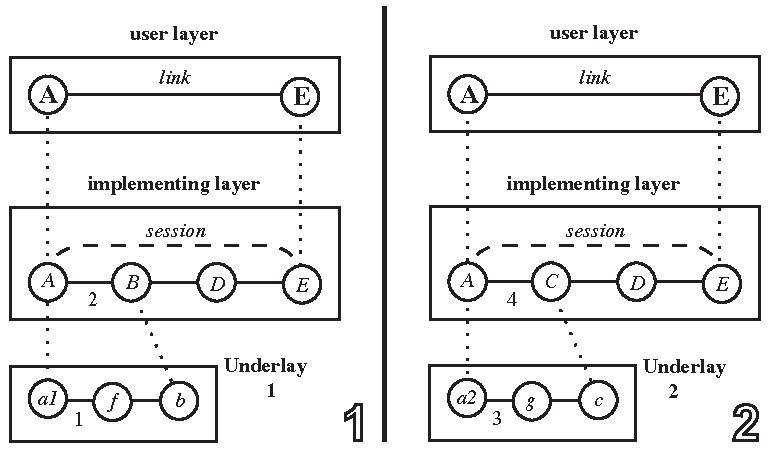
\includegraphics[scale=0.95]{figures/drm.pdf}
\caption{Two stages in an instance of dynamic-routing mobility.}
\label{fig:drm}
\end{figure}

The precise site of mobility here is the lower endpoint {\it A}.
In Stage 1 {\it A} is registered at {\it a1} in
Underlay 1.
{\it a1} and {\it A} are connected to the rest of their layers
through Links 1 and 2, respectively.  
Link 2 is implemented by Underlay 1.

Between Stage 1 and Stage 2
Link 1 stops working, possibly because the machine on which
{\it A} and {\it a1} reside has
been unplugged from a wired subnetwork, or
has moved out of range of a wireless subnetwork.
In a cascading sequence of events, 
Link 1 is destroyed,
Link 2 is destroyed, and the registration
of {\it A} at {\it a1} is destroyed. 
{\it A} is now disconnected from the rest of its layer.

Eventually the mobile machine may become plugged into another
wired subnetwork
or enter the range of another wireless subnetwork, as shown in Stage 2.
In a cascading sequence of events, member {\it a2} (which is
the mobile machine's member in the new Underlay 2)
connects to the rest of its layer through Link 3,
{\it A} becomes attached to new location {\it a2}, and new Link 4 is
created in the mobility layer and implemented by Underlay 2.
Note that {\it A} is now linked to {\it C} rather than {\it B};
this change is necessary because {\it C} is attached to Underlay 2 and
{\it B} is not.

Between Stages 1 and 2 there may be an interval during which {\it A}
has no connection with the rest of its layer.
There may also be an interval in which Stages 1 and 2 overlap, so
that {\it A} is temporarily attached to both underlays.

The hard problem to be solved in Figure~\ref{fig:drm} is that 
even after {\it A} is again reachable by other members of its layer
such as {\it D} and {\it E}, they do not know how to find it because
the routes to it are obsolete.
{\it Dynamic-routing mobility} relies on the routing algorithm of
the layer, which must learn about new links, recompute routes,
and update forwarding tables.
After this is accomplished, {\it D} will know that it can reach
{\it A} by forwarding to {\it C}.

There are three ways in which actual dynamic-routing
mobility can differ from the
example in Figure~\ref{fig:drm}.
Fortunately, none of them affect what the implementation has to do,
so none of them need be discussed separately.
First, the new attachment {\it a2} could be in the same layer as 
{\it a1}, rather than in a different layer.
Because {\it a1} and {\it a2} are different locations,
after the move {\it A} is probably linked to
a different member of its own layer, even though the new link is
implemented by the same lower layer as before.

Second, in Figure~\ref{fig:drm} the mobile member {\it A} has only
one attachment and one necessary link.
As shown in Figure~\ref{fig:scope}, members such as gateways have
multiple simultaneous attachments to different underlays.
Because each such attachment is necessary for the gateway's
purpose and supports its own link or links,
the mobility of each attachment is a separate problem to be solved.

Third, occasionally a layer implements sessions for the benefit of
its own members, rather than as a service to a higher user layer.
In this case there is no {\bf A} or {\bf E}, and the beneficiaries of
the mobility implementation are {\it A} and {\it E}.

A {\it router} is a member of a layer that receives and forwards messages
not destined for itself, whether it sends and receives messages on its
own behalf or not.
A {\it forwarding table} is a distributed copy of some of the
{\it routes} state component of a layer.
Implementations of dynamic-routing mobility incur four kinds of
resource cost:
\begin{itemize}
\item
{\it storage cost} is the cost of storing routes to mobile members,
in the forwarding tables of all the routers that need them;
\item
{\it update cost} is the cost of updating the stored routes as mobile
members move;
\item
{\it path cost} is the cost of longer or more congested message paths
due to mobility;
\item
{\it handoff latency} is the message delay caused by a move.
\end{itemize}
These costs will be discussed further in 
Section~\ref{sec:majordifferences}.

The primary issue in implementing dynamic-routing mobility (DRM) is
that large layers such as the classic Internet core achieve scalability
through a hierarchical name space.
In the Internet core, names (IP addresses) are organized into a
hierarchy based on geographical, topological, and administrative
factors.
A layer member is assigned a name based on its location in this hierarchy.
Subtrees in the hierarchy correspond to blocks of names, and routing
scales because it operates on aggregated
blocks rather than individual names.
Mobility violates the rules of this scheme, because a mobile member
retains its name as it moves across the boundaries of the hierarchy.
If implemented naively, it would require a large number of entries
in the forwarding table of each IP router for individual mobile machines.

This issue is so important that the design decisions made to implement
DRM are completely different in hierarchical and non-hierarchical
layers.
For that reason, we have divided examples of DRM into two sections
(Sections~\ref{sec:sec4} and \ref{sec:sec5}).

\subsection{Session-location mobility}
\label{sec:slm}

Figure~\ref{fig:slm} has the same two stages as Figure~\ref{fig:drm}.
The most important
difference is that {\bf A}'s location in the implementing
layer changes from {\it A1} to {\it A2}, rather than staying the same
as it did in Figure~\ref{fig:drm}.
In geomorphic terms, the mobile machine's representative in the
implementing layer (with name {\it A1}) has died, and has been reborn
as a member of the implementing layer with name {\it A2}.

\begin{figure}
\centering
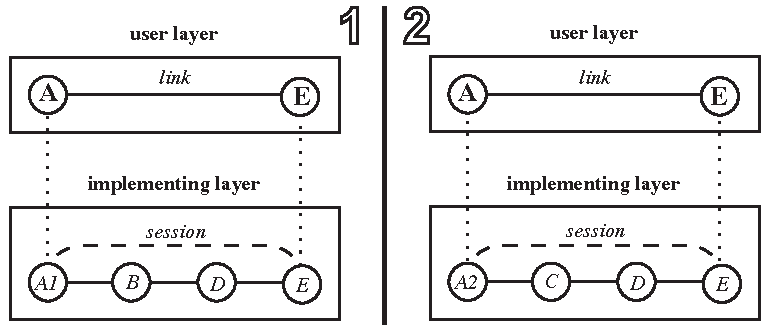
\includegraphics[scale=0.95]{figures/slm.pdf}
\caption{Two stages in an instance of session-location mobility.}
\label{fig:slm}
\end{figure}

This is a natural occurrence in a layer with a hierarchical name
space.
It should be 
familiar from observing what happens
when a laptop with an IP address {\it A1} moves to a new subnetwork
of the Internet, and gets a new IP address {\it A2} from DHCP.
The laptop cannot continue to use {\it A1} in the new subnetwork,
because {\it A1} is not in the subnetwork's address block.

DHCP alone is not sufficient to implement mobility, however.
As explained in Section~\ref{sec:layers.and.mobility}
and shown in Figure~\ref{fig:slm},
the strongest form of mobility requires preserving the 
communication channel in the user layer.
The bulk of the work of implementing session-location mobility lies in 
ensuring that {\bf A}'s correspondents know that it is now located at
{\it A2} rather than {\it A1}.
Each lower endpoint that was participating in a session with {\it A1}
on behalf of {\bf A} must be informed that it should now be corresponding
with {\it A2} instead.

As explained in Section~\ref{sec:layercomponents},
when an underlay is implementing a channel for an overlay, the initiating
lower endpoint must be able to look up the location of the 
accepting higher endpoint in the underlay, so that it can send messages
to it.
This means that there must be a globally accessible copy of the
{\it locations} mapping in the layer.
Session-location mobility also requires updating this mapping when
a higher endpoint moves.

Generally the fastest handoffs are achieved when a new lower endpoint
sends updates directly to all its correspondent lower endpoints
(in addition to updating the {\it locations} mapping).
This requires, of course, that the new lower endpoint have the 
correct name of the lower endpoint at the other end of each session.

Interesting behavior arises if both ends of a session move 
concurrently.
Neither lower endpoint will know the new name of the far endpoint,
so neither can send an update to the other.
In this simultaneous handoff
scenario a mobile endpoint, finding that it cannot reach a far
endpoint to update it, will suspect that the far endpoint has moved also.
Both endpoints must fall back on lookup from the {\it locations}
mapping to get the new location of the far endpoint.

As with Figure~\ref{fig:drm}, the two stages in Figure~\ref{fig:slm}
might have a gap between them or might overlap.
If they overlap, there will be an interval during which {\it A}
has two attachments in the same layer.

In Figure~\ref{fig:slm} the underlays are not shown,
although they probably look similar to those in Figure~\ref{fig:drm}.
Most likely there is an underlay member
{\it a1} that is destroyed, 
and an underlay member {\it a2} that is created.
There is no mobility observable at this level, however, because 
{\it A1} is attached to {\it a1} in Underlay 1 throughout its lifetime, and
{\it A2} is attached to {\it a2} in Underlay 2 throughout its lifetime.
The only mobility that is observable is {\bf A}'s change of attachment
from {\it A1} to {\it A2}.

Strictly speaking some dynamic routing could be involved in
session-location mobility, because
{\it A2} is a new member of the layer and there must be routes to it.
In practice this is rarely an issue, because the name
{\it A2} is part of some
larger block to which routes already exist.

Like DRM, session-location mobility (SLM) has storage costs,
update costs, and handoff latency.
The storage costs are the costs of maintaining a 
scalable implementation of {\it locations}.
The update costs are the costs of updating {\it locations} and
current correspondents when a member moves.

Implementations of SLM vary in a number of ways
(see Section~\ref{sec:sec6}),
although no one variation is as important as the hierarchical {\it versus}
non-hierarchical
variation for DRM.

\subsection{Major differences between the patterns}
\label{sec:majordifferences}

There are obvious structural differences between the two patterns:
\begin{itemize}
\item
In DRM the change of attachment appears between the implementing layer
and the level 
below it, while in SLM the change of attachment appears between
the user layer and the implementing layer 
(see Figures~\ref{fig:drm} and \ref{fig:slm}).
\item
In DRM the bulk of the work is performed by the routing algorithm,
while in SLM the bulk of the work is performed by the session protocol
and location algorithm (see Figure~\ref{fig:table}).
\item
In DRM the major state components that change are {\it attachments, links,}
and {\it routes} 
(see Figure~\ref{fig:table}).
In SLM the major state components that change are {\it locations}
and {\it sessions}. 
\end{itemize}
These structural differences prove that the two patterns are
fundamentally different.

In attempting to understand mobility mechanisms, people are sometimes
confused by the fact that {\it routes} (changed by DRM) and 
{\it locations} (changed by SLM) are both mappings.
The {\it locations} mapping is usually implemented by a shared global
data structure called a
{\it directory}.
The {\it routes} mapping is usually distributed across the forwarding
tables of the routers, but is occasionally implemented as a directory.
The result is that directories are sometimes used in both DRM and SLM
implementations.

This similarity is superficial because it does not tell
us the most important thing about
these mappings, which is what they mean in terms of
network architecture.
The mappings used in DRM and SLM are always fundamentally different, and
can always be distinguished from one another.
As mentioned in Section~\ref{sec:drm},
{\it routes} is a peer-to-peer or intra-layer mapping:
at each router, entries in the forwarding
table map each destination name to a member, link, or path {\it in the
same layer}. 
{\it Locations}, on the other hand, is always an inter-layer mapping,
mapping names in a higher layer to names in a lower layer.

In describing mobility mechanisms, people often focus on the
``identifier-locator split.''
This may be useful intuition, but should be interpreted carefully.
In an episode of mobility there is always a layer member that retains
its identity (the ``identifier''), and two members at a lower level,
where the attachment of the identifier moves from one to the other
(the ``locators'').
The identifier-locator split
does not distinguish DRM from SLM, although in the two patterns
the identifiers and locators appear at different levels.
In addition, it is important to remember that these terms are
relative, as mobility can occur anywhere in a layer hierarchy. 

On the surface, it may seem that DRM should be called ``in-network
mobility'' or the like, while SLM should be called ``end-to-end mobility''
or the like.
This reflects a misunderstanding of how general the patterns are,
and how freely they can be applied at different levels.
For one example, consider an application layer whose members run
only on Internet
hosts.
The members include user clients and named services.
The layer could have its own dynamic,
application-specific routing to services,
which allows services to be reached even though they move from server
to server.
This instance of DRM is not ``in network'' from most peoples' perspective.
For another example, an Internet router might itself be mobile,
and might have some of its links to other Internet routers
preserved as it moves by session-location
mobility at a lower level.
This instance of SLM does not involve any endpoints according to most
peoples' perspective.

Obviously a quantitative comparison between two mobility implementations
cannot be made without implementation details and a profile of the
expected load.
Nevertheless, it is possible to make some general comparisons
between the two patterns based on their potential strengths and 
weaknesses.
We say ``potential'' because any characteristic, whether positive or
negative, can be irrelevant in some situations.

The greatest potential
weakness of DRM is its storage, update, and path costs.
Normally routing information is different in different places,
so there is a lot of it, it is spread widely across a layer, and it
is expensive to update.
Attempts to economize on storage and update costs can lead to high
path costs (see Section~\ref{sec:sec5}), as messages travel further
to be routed successfully.
Path costs must be weighted heavily because {\it every}
message that travels on a
channel is affected by its path cost, if any.

Locations are very different from routes because the result of a location
query is usually the same no matter which member is querying (in
contrast to a route, which is different depending on where it is
starting from), and because a location query is needed only at the
beginning of a session and possibly after a move (in contrast to routes,
which are consulted on every hop of every message).
As a result, locations can be stored and updated much more cheaply
than routes.
For example, even a centralized directory would perform adequately
in many contexts.
And even if lookup of a location is slow, we do not count it as a
path cost because the cost is incurred a few times for each channel
rather than 
being built into the cost of transmitting each message on the channel.

The greatest potential
weakness of SLM is that it must be implemented with
the participation of session endpoints.
This means that deployment of an SLM mechanism requires new or
upgraded mobile devices that run the SLM protocol for sending and
receiving location updates.
Full interoperation with legacy endpoints calls for expensive middleboxes.
Security is a concern because endpoint devices can initiate
updates of the global layer state.

Concerns such as software upgrading and security have attracted less
attention with respect to DRM.
This is because a layer can, in principle, be designed so
that its members are partitioned into endpoints and routers, and
only the routers need be aware of or participate in an implementation
of DRM.
In reality these concerns are ubiquitous in distributed computing, and
can apply to routers as well.


% This work is licensed under
% http://creativecommon.org/licenses/by/3.0/
\section{Examples of dynamic-routing mobility in non-hierarchical layers}
\label{sec:sec4}

Dynamic-routing mobility is often used in LANs, which have smaller
scopes and can function without a hierarchical name space.  
%
% JEN: Pamela, check this
%
These LANs handle mobility naturally as part of the normal routing
function, since end-points retain their addresses as they move and
routing does not rely on location-dependent addressing.

\subsection{Wired Ethernet LANs}

An Ethernet LAN is a single layer.
Its member processes are the Ethernet representatives of hosts (endpoints)
and switches (routers),
and its names are MAC addresses.
It has no pre-attachment requirements or configuration for hosts,
which makes it ``plug and play.''

The LAN offers both broadcast and point-to-point services to
higher layers.
In this brief section we do not consider these communication services
further, so
there will be no discussion of the layer's sessions or locations.
Also, for simplicity, we will not extend the modeling into lower levels,
so links in the Ethernet layer are primitives.

An Ethernet layer has two kinds of links.
There are point-to-point links between 
switches, each of which is basically a wire
between two machines.
There are also shared media or buses.
A bus delivers each message
to every machine on the bus, and is used to connect a switch to a
set of hosts.
Either kind of link
can be identified at each switch that
uses it by the port on the switch's machine to which it is attached.

The inter-switch links of the layer must form a bidirectional
spanning tree (see Figure~\ref{fig:ethlinks}). 
Otherwise, when flooding is used (see below), 
the network could be overwhelmed by
messages traveling on cycles.
There are usually more physical links than needed for the spanning tree,
but the extras
can only be used when other links fail and the spanning tree
is recomputed.

\begin{figure}
\centering
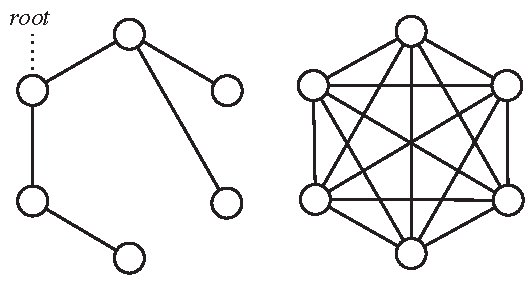
\includegraphics[scale=1.00]{figures/ethlinks.pdf}
\caption{Inter-switch links of an Ethernet LAN layer (left) and an overlay
layer (right).
The Ethernet links are physical, while the overlay links are virtual.}
\label{fig:ethlinks}
\end{figure}

Each switch has a forwarding table containing {\it (MAC address, port)}
pairs.
The port identifies the link on which the switch should forward messages
destined for the MAC address.  
Each switch's table is sparse and is populated lazily by a routing
algorithm called ``MAC learning.''
Upon receiving a message with a source MAC 
address that is not in its forwarding
table, the switch adds to its table the MAC address and the link
on which the message was received.

The forwarding algorithm of a switch is similarly simple.
Upon receiving a message not destined for itself, the switch looks for the
destination MAC address in its own forwarding table.
If it finds an entry, it forwards the message on the designated link.
If it does not find an entry, it ``floods'' by forwarding the message
on every link except the one on which it was received.

These mechanisms implement dynamic-routing mobility as an
aspect of normal operation rather than as a special case.
When a host moves within the layer, it changes the link through which
it is attached to the layer.
As soon as it sends messages, new routes to it begin to propagate through
the layer.
Obsolete forwarding-table entries
are removed when their time-to-live expires.
Missing table entries are handled by flooding.
Note that an entry might also be removed from a forwarding table because
the table is full and space for a newer entry is needed.

\subsection{Ethernet overlays}

Several recent
designs~\cite{seattle,vl2,nvp} avoid flooding by forming
an overlay topology that interconnects all of the edge switches, as
shown on the right side of Figure~\ref{fig:ethlinks}.  While the
inter-switch links of an Ethernet are physical and form a spanning
tree, the inter-switch links of an overlay network are virtual and
fully connect the switches.  

The virtual links are communication services implemented by a second,
lower layer.  For example, Figure~\ref{fig:seattle} shows the path of
a message from host {\it Hv} to host {\it Hz} (the lower-case letters
stand for their MAC addresses).  On each hop, the path is labeled with
the source name above and the destination name below.  The virtual hop
between switches {\it Sw} and {\it Sy} in the overlay layer is
implemented in the underlay, where the message is encapsulated in a
message with source {\it w} and destination {\it y}.

How are the virtual links in the overlay implemented by the underlay?
The members of the underlay layer are the switches
only, not the hosts.  Each switch's name is the MAC address of its
machine, just as in the overlay, so there is no need for a 
{\it locations} state component to map one name to another.  
The members of the underlay are stable and
stationary.  Routing is static except for failures, and the forwarding
tables are fully populated.  Because there is no flooding, there is no
need to restrict the links to a spanning tree, and all of the physical
links between switches can be fully utilized.  
The underlay can run an efficient routing protocol, such as a link-state
protocol, to compute a shortest path from one edge switch to
another.

\begin{figure}
\centering
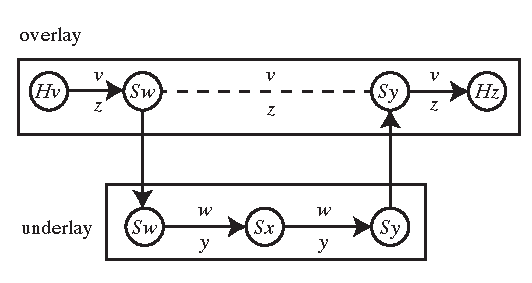
\includegraphics[scale=1.00]{figures/seattle.pdf}
\caption{The path of a message through two layers and three
switches.}
\label{fig:seattle}
\end{figure}

Routing in the overlay is unusual compared to routing in general,
because every edge switch is directly linked to every other edge switch.
This means that an inter-switch route to a host
can be identified simply by the
MAC address of the host's edge switch, and is exactly the same
no matter which switch needs the route!
Thus inter-switch routing is a mapping that is {\it global}
within the layer.
%
% JEN: Pamela, check this
%
Note that, despite the use of a single global directory, the mapping
performed is indeed part of \emph{routing} within the layer (i.e., the
{\it routes} mapping), \emph{not} a {\it locations} mapping between
two layers.  The underlay layer in Figure~\ref{fig:seattle} exists to
make the \emph{routing} between the edge switches more scalable, not
to implement the \emph{link} between the two end-points.

As with Ethernet LANs, each switch has a routing table that is
populated lazily ({\it e.g.}, through MAC learning).
The difference lies in what happens when a switch needs a route to
an unknown destination.
Rather than flooding, it looks the route up in a global routing
directory.

When a host moves, the directory is
updated with the new route to the host.  The exact update mechanism
differs from one overlay design to another, depending on whether
mobility is planned ({\it e.g.,} 
virtual-machine migration in a data center)
or unplanned ({\it e.g.,} a mobile device moving within a campus).  In a
data center, a central controller that triggers virtual-machine
migration can also update the directory with the new
route~\cite{vl2,nvp}.  If the directory cannot be informed in advance
that a host is moving, the new local switch can learn that a new
device has connected and subsequently update the
directory~\cite{seattle}.

The routing directory in an overlay is an important part of its design, 
and may have
many features to make both queries and updates fast and efficient.
Different designs have different directory structures.  VL2~\cite{vl2}
and NVP~\cite{nvp} run a centralized directory on a collection of
server machines.  In these designs, if the ingress switch {\it Sw}
does not know the route for host {\it Hz}, {\it Sw} queries a
directory server to learn the route {\it Sy}.  In contrast,
SEATTLE~\cite{seattle} implements the directory as a ``one-hop
Distributed Hash Table''~\cite{gupta} running directly on the
switches.  
If the ingress switch {\it Sw} does not know the route for
host {\it Hz}, {\it Sw} computes the hash of the {\it Hz}'s MAC
address and forwards the message over a single overlay link to the
switch responsible for this hashed value.  This switch, in turn,
forwards the message to {\it Hz}'s local switch {\it Sy} and informs
switch {\it Sw} of the route for {\it Hz} so that future messages flow
directly from {\it Sw} to {\it Sy}.

To improve the speed of mobile handoff, the ingress switch {\it Sw}
can receive an update when a host moves to a new location.  To perform
these updates, the directory could maintain information about all
ingress switches that recently queried the directory for a route to
{\it Hz}.  However, this can require the directory to maintain a large
amount of state.  Instead, when a host moves, the directory can update
the mobile host's old local switch.  Upon receiving a message for the
mobile host, the old local switch can both forward the message to the
mobile host and send an immediate notification about the new route to
the sending switch~\cite{seattle}.  This reactive invalidation of
stale routes obviates the need for the directory to maintain
information about which ingress switches sent queries for {\it Hz},
while still ensuring rapid invalidation of stale routes.

In addition to SEATTLE, VL2, and NVP, several other designs adopt
certain aspects of the overlay solution.  
The early work on
Rbridges~\cite{rbridges}, and the resulting TRILL~\cite{rfc5556}
standard at the IETF, also forms an Ethernet overlay with
shortest-path routing in the underlay.  
However, instead of having an
explicit directory service, TRILL relies on flooding to reach hosts
with unknown routes.  
Rather than flooding on all normal overlay links, TRILL floods
on a special multicast link in the overlay.
This special link is implemented in the underlay by a multicast tree
formed on the underlay topology.

Like VL2 and NVP, the PortLand~\cite{portland} design
has a set of directory servers that allow ingress switches to learn
the route to a destination host.  Instead of encapsulating a message,
PortLand assigns each edge switch a block of host ``pseudo-MAC
addresses'' and rewrites the host MAC addresses at the edge.  To
enable the use of hierarchical pseudo-MAC addresses, PortLand is
restricted to the tree topologies common in data-center networks.
Table~\ref{tab:overlays} summarizes the structural characteristics
of all five designs.

\begin{table}
\begin{center}
\begin{tabular}{|l|l|l|} \hline
\multicolumn{1}{|c|}{\bf Protocol} &
 \multicolumn{1}{c|}{\bf Routing Directory} &
 \multicolumn{1}{c|}{\bf Encapsulation} \\ \hline
SEATTLE &
 one-hop DHT on the switches &
 simple encapsulation \\
VL2 &
 directory servers &
 simple encapsulation \\
NVP &
  directory servers &
  simple encapsulation\\
Rbridges/TRILL &
  none, flooding on multicast tree &
  simple encapsulation\\
PortLand &
 directory servers &
 none, MAC rewriting\\
\hline 
\end{tabular}
\end{center}
\caption{Ethernet overlay designs for dynamic-routing mobility.}
\label{tab:overlays}
\end{table}

\subsection{Comparative resource costs}
\label{sec:props}

Concerning storage costs, both Ethernet LANs and overlay designs
incur the costs of the
forwarding tables in switches.
These costs are kept moderate by the fact that the tables are sparsely
populated.
Because there is no aggregation of names or table entries, the costs
of densely populated tables would be too great.
In addition to the forwarding tables, the overlay designs incur a storage cost
for the routing directory, which maintains global state for the layer.

Concerning update costs, both approaches incur negligible costs for 
populating forwarding tables lazily through MAC learning.
The biggest update cost is the cost of Ethernet flooding.
The cost of flooding, in terms of bandwidth, grows quadratically with the
size of the network---which makes it a potential scalability problem.
Whether it becomes an actual problem or
or not depends on its frequency, which
depends on both the frequency of moves and the number of correspondents
that a mobile host tends to have.
SEATTLE, VL2, NVP, and PortLand have no flooding cost, though
they do have the additional cost of updating the directory.

Mobility in the overlay designs incurs no path cost.
The path cost of Ethernet mobility is significant, because the spanning
tree (which is necessitated by flooding) forces paths to be longer and
forces some physical links to go unused.

We can measure handoff latency from the instant when the mobile host
re-attaches to the network and informs its local switch (before that
time no mobility mechanism can take effect).
The following scenarios assume that a correspondent switch is sending
a steady stream of messages to a mobile host.
They describe the elapse of time before messages sent by the
correspondent switch (CS) are forwarded to the mobile host at its new
attachment.

The Ethernet scenario:
\begin{enumerate}
\item
The time-to-live of the CS's route to the mobile host expires, if it has
not already.
\item
CS receives the next message from the correspondent host and floods it.
\item
After a round trip to the mobile host, CS learns the new route.
\end{enumerate}
After Step 3, messages sent by CS are forwarded to the mobile host at
its new attachment.

In the directory-based overlay solutions ({\it i.e.,}
SEATTLE, VL2, NVP, and PortLand):
\begin{enumerate}
\item
The directory receives an update of the mobile host's new local switch.
\item
The directory informs the mobile host's old local switch of the new route.
\item
The next message arrives at the mobile host's old local switch, and
is forwarded on the new route.
\item
The mobile host's old switch also informs the CS of the new route.
\end{enumerate}
At Step 3 and after, messages sent by CS are forwarded to the mobile
host at its new attachment.
If Step 1 of the Ethernet scenario takes time, then the handoff latency
of the overlay designs will be smaller than the Ethernet's.

In addition to resource costs,
security and privacy are ever-present concerns.
In Section~\ref{sec:majordifferences} we noted that DRM usually
has minimal security problems because only routers participate
in routing.
Ethernet flooding is an exception to this rule because 
it allows hosts to play a role in routing.
Malicious
hosts can force flooding by filling up the network's forwarding tables.
(This would be accomplished by sending many messages from spoofed
source MAC addresses.)
Severe flooding can cause denial of service.
Also, the
malicious hosts will receive all the flooded packets, which
may contain private information that they wish to see.


% This work is licensed under
% http://creativecommon.org/licenses/by/3.0/
\section{Examples of dynamic-routing mobility in hierarchical layers}
\label{sec:sec5}

Both of the designs in this section are intended for mobility within
the Internet core.  For this reason, both must grapple with the
problem of a hierarchical name space as explained in
Section~\ref{sec:drm}.
To reduce overhead, both solutions
significantly limit the number of routers in the Internet that must
store and update state concerning how to reach each mobile node.

\subsection{Mobile IPv4}
\label{sec:mipv4}

Mobile IPv4 \cite{mobile-IP,rfc3344} drastically reduces storage and update
costs by reducing the number of routers that must have a current route
to a particular mobile host to one or two.
Also, because each router is responsible for only a limited number of
mobile hosts, no router is over-burdened by mobility.

Figure~\ref{fig:mipv4} shows the path of a message from correspondent
host {\it C}
to mobile host {\it M} in an Internet core layer with Mobile IPv4.
Router {\it HA} is the {\it home agent} of {\it M}, and is supposed to
have a route to it at all times.
Router {\it FA} is the {\it foreign agent} of {\it M}, meaning that
it is local to the subnetwork where {\it M} is now attached,
and currently knows a route to {\it M} through the subnetwork.

\begin{figure}
\centering
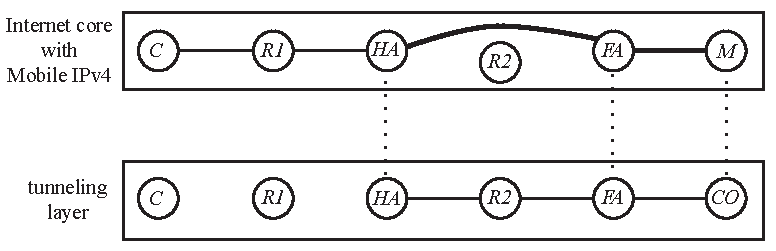
\includegraphics[scale=0.90]{figures/mipv4.pdf}
\caption{The path of a message to mobile host {\it M} with Mobile IPv4.
Special links are drawn with heavier lines.
Only the links employed in the path are shown.}
\label{fig:mipv4}
\end{figure}

The IP address {\it M} is in an aggregated routing block such that
all messages destined for the block are routed to {\it HA}.
Thus this router need only be the home agent for mobile hosts with
IP addresses in its
block.
The message from {\it C} arrives at {\it HA} by means of normal IP
routing through router {\it R1}.
The subnetwork of {\it HA} is {\it M}'s home subnetwork, so when {\it M}
is at home {\it HA} has a local route to it.

When {\it M} is not at home and becomes
attached to the subnetwork of {\it FA}, it gets a local ``care-of''
IP address {\it CO}
in that subnetwork.
{\it M} informs {\it FA},
which informs {\it HA} that it is the current foreign agent of {\it M}.
To forward messages to {\it M}, however, {\it HA} cannot merely forward
them toward {\it FA}.
It they were sent out on normal IP links, normal IP routing would send
them back to {\it HA}!
Messages to {\it M} from {\it HA} and {\it FA} must be forwarded on
special links that are separate from normal IP links.

As shown in Figure~\ref{fig:mipv4}, the special links in the Internet
core are implemented by a tunneling layer below the core layer.
The home agents, foreign agents, and mobile hosts of the Internet core
are all registered at members of the tunneling layer.
Home agents and foreign agents have the same names in both layers,
while
{\it M} is attached to member {\it CO} in the tunneling layer.
To forward a message for {\it M}
on its special link, {\it HA} in the core layer encapsulates the
message in another message destined for {\it FA}, and passes the message
to member {\it HA} in the tunneling layer.

Although the tunneling layer resembles the core layer (see below), 
its state differs from that of the core layer in several important 
respects:
\begin{itemize}
\item
{\it Routes:}
In the core layer, 
at {\it HA} messages for {\it M} are forwarded to {\it FA} on a special 
link,
at {\it FA} messages for {\it M} are forwarded to {\it M} on a special 
link,
and everywhere else messages for {\it M} are forwarded to {\it HA} on 
a normal link.
In the tunneling layer {\it M} does not exist.
\item
{\it Attachments:}
Some
members of the core layer are attached to members of the tunneling layer.
\item
{\it Locations:}
The core layer has no {\it locations} state, at least not related to
Mobile IPv4.
Although the tunneling layer need not maintain explicit
{\it locations} state for
mobile routers because they have the same names in both layers,
it must maintain explicit {\it locations} state for mobile hosts from the
core layer.
This state, which supplies the current local IP address of a mobile host,
is stored in the foreign agent to which it is relevant.
\end{itemize}

In Mobile IPv4, mobile hosts such as {\it M} send messages to their
correspondents such as {\it C} though normal IP links.
This often creates problems because IP address {\it M} is not part of
the normal routing block of the subnetwork at {\it FA}.
If there is ingress filtering for security in or near this subnet,
messages with a source address of {\it M} will be thrown away.
In Section~\ref{sec:sec7} we shall see how Mobile IPv6 eliminates this
problem.

Overall this is an interesting architecture because 
the Internet core layer and the tunneling layer
are mostly identical, and share the same
implementation.
Home agents, foreign agents, and mobile hosts are all aware of the
differences between the layers and aware of their dual membership and
dual roles.
The shared implementation works because none of the other members
of the layers need to be self-aware in that way.
They always behave the same, without knowing that sometimes their
actions contribute to the core layer, while other times their actions
contribute to the tunneling layer.

By distinguishing clearly between the two layers,
we make it possible to check the correctness of the software for each.
It also becomes possible to make further distinctions if advantageous.
For instance, implementation of a
link between {\it HA} and {\it R2} can be shared by
both layers, but it might make sense to distinguish links in the two
layers for reasons of performance or accounting.

\subsection{MSM-IP}

MSM-IP \cite{multicast} is a proposal for using IP multicast
to implement mobility.
A mobile host gets an IP address {\it M}
in the distinguished multicast block.
When the mobile host
attaches to a new subnetwork using local IP address {\it L},
{\it L} joins the multicast group for {\it M}, and the previous
local address used by {\it M} resigns from the group.

With IP multicast there is a distinguished set of multicast routers,
which are globally distributed and 
are responsible for routing messages destined for a multicast
address to all members of the address's current multicast group.
These routers exchange information and forward messages to each other
through special links,
exactly as the routers participating
in Mobile IP do.
The special links are implemented by a tunneling layer, exactly as the
special links in Mobile IP are.

With MSM-IP, every subnetwork that supports either mobile hosts or
their correspondents must have a multicast router.
Messages to mobile hosts (or true multicast groups) are recognized
by their distinguished addresses and sent to their local multicast
router, where they enter the special multicast routing 
system.

\subsection{Comparative resource costs}

The costs of dynamic-routing mobility depend greatly on the number
of routers that must have a current route to each mobile host.
More routers incur more storage and update costs.
Storage and update costs are much greater for MSM-IP than for Mobile IPv4,
because an entire network of multicast routers must be updated on each
move.

Using fewer routers, on the other hand, incurs more path cost.
With MSM-IP path cost is minimal, because a message travels from the
multicast router in the sender's subnetwork, along an optimal path 
through the distributed multicast routers, to the multicast router in
the receiver's subnetwork.
With Mobile IPv4 path cost can be high, because each message to a mobile
host must pass through the home agent, regardless of where the sender
is and where the mobile host is.
This problem of path cost or ``triangular routing'' is the reason why
the designers of Mobile IPv4 decided to send messages from mobile hosts
through normal IP links.
They incur no path cost, but they do run afoul of security
filtering.\footnote{Messages from MSM-IP mobile hosts do not have
problems with security filtering because multicast IP addresses are
recognizable as belonging to a special category.}

In Section~\ref{sec:majordifferences} we said that dynamic-routing
mobility does not in principle require participation of the endpoints.
Mobile hosts in Mobile IPv4 and MSM-IP do not have this advantage.
The reason that they must have special behavior is that both designs
use special routing mechanisms, separate from normal IP
routing, to find mobile hosts.
Because the routing mechanism is special, it is not necessary to
update every IP router when a mobile host moves.
But also, because the routing mechanism is special, mobile hosts must also
behave differently to interact with it in the correct way.


% This work is licensed under
% http://creativecommon.org/licenses/by/3.0/
\section{Examples of session-location mobility}
\label{sec:sec6}

In this section we compare four proposals for session-location
mobility: the
Host Identity Protocol (HIP)~\cite{RFC-4423,HIP}, 
the Identifier-Locator Network Protocol (ILNP) \cite{ILNP1,ILNP2},
the
Locator/Identifier Separation Protocol (LISP) Mobile Node~\cite{LISP-MN}, 
and the ``route optimization'' mechanism of Mobile 
IPv6 \cite{mipv6old,mipv6new}
(Section~\ref{sec:mipv6} will explain how route optimization fits into
Mobile IPv6 overall).
All but ILNP are IETF standards, and ILNP has resulted in many
IETF documents with ``experimental'' status.

These proposals have many similarities, as
they all provide mobility by splitting 
the Internet core layer (shown in Figure~\ref{fig:scope}) into two
layers.
These two layers 
are shown in Figure~\ref{fig:identloc}, and also correspond to
the two layers in Figure~\ref{fig:slm}.
SLM supports the persistence of inter-layer channels that are
links in the upper layer and sessions in the lower
layer.\footnote{Note that the members of the
identifier layer are {\it hosts}, while the members of the locator
layer are {\it interfaces}.
This distinction can safely be ignored in this section, but it is
important for multihoming as discussed in Section~\ref{sec:multihoming}.}

\begin{figure}
\centering
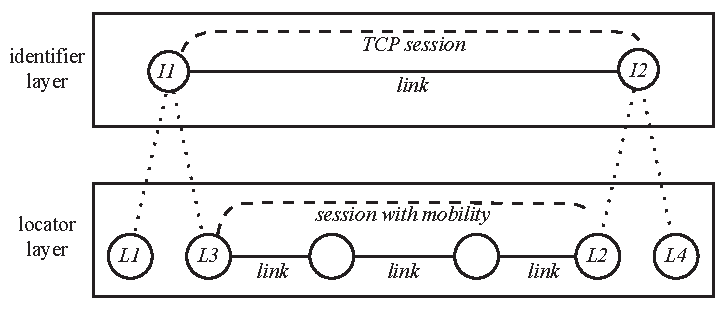
\includegraphics[scale=0.80]{figures/identloc.pdf}
\caption{The Internet core layer splits into two layers for
well-known examples of session-location mobility.  
In the identifier layer, session protocols such as TCP run
largely unmodified.
In the locator layer, the session protocol implements mobility.}
\label{fig:identloc}
\end{figure}

In an attempt to use a widely acceptable common terminology,
we call the upper layer 
the {\it identifier layer}, and the lower layer
the {\it locator layer}.
Names in the two layers are referred to as {\it identifiers} and
{\it locators}, respectively.
This common terminology does not necessarily match the terminology
typically used to explain each specific protocol.

Note that
Figure~\ref{fig:identloc} is an approximation of the real
implementations of these standards, in which the split between layers may
be implicit or incomplete.
In the geomorphic view, two separate session protocols are employed.
In the identifier layer, a largely unmodified TCP implementation provides
the usual TCP service as if identifiers were IP addresses.
(UDP and other service protocols operate here 
as well.)
In the locator layer, the only purpose of the session protocol is
to implement SLM.

\subsection{Names}

Table~\ref{tab:slm} compares the four proposals on their choices of
names.
They differ most on identifiers, which must be globally unique and
persistent, but have no other necessary constraints.

\begin{table}
\begin{center}
\footnotesize
\begin{tabular}{|l|l|l|} \hline
\multicolumn{1}{|c|}{\bf Protocol} & 
  \multicolumn{1}{c|}{\bf Identifier} & 
  \multicolumn{1}{c|}{\bf Locator} \\ \hline
HIP & (hash of) public key & IPv4 or IPv6 address \\ \hline
ILNPv6 & 64-bit IPv6 suffix & IPv6 address \\ \hline
LISP Mobile Node & IPv4/IPv6 address (called EID) & IPv4/IPv6 address (called RLoc) \\ \hline
Mobile IPv6 & IPv6 address & IPv6 address \\ \hline
\end{tabular}
\end{center}
\caption{Comparison of SLM proposals on the basis of names.}
\label{tab:slm}
\end{table}

HIP places a great emphasis on building in security, so the identifier
of a host is the host's
public cryptographic key.
With the use of keys as identifiers, 
messages can have self-authenticating source information.
Self-authentication provides security within the SLM locator
update protocol (see Section~\ref{sec:updateprotocols}), while
the guaranteed presence of a public key makes it easy to protect
the channel data with encryption.
Identifiers can also be hashes of public keys, which allows for shorter
identifiers without sacrificing self-authentication.

ILNPv6 is the IPv6 version of ILNP.
Its identifiers are 64 bits long; a host usually chooses a unique
identifier for itself
by taking the 48-bit MAC address of one of its hardware
interfaces and using a standard algorithm to extend it to 64 bits.

The significance of 64 bits is that in IPv6 routing based on 
hierarchical names and aggregation, the longest possible prefix is
64 bits.
This means that at its finest-grained, IPv6 routing examines the
first 64 bits of an IPv6 address and points to a
subnetwork.
The IPv6 address still has a 64-bit suffix to map to an IPv6 interface
attached to the subnetwork.
In ILNPv6, 
identifiers are carried in the 64-bit suffixes of IPv6 addresses.
In other words, an ILNPv6 locator is derived from an ILNPv6 identifier
by prefixing 64 bits that indicate a subnetwork where the identified
host can be found.\footnote{This is different from ILNP terminology,
in which the 64-bit prefix is itself the ``locator.''} 
This scheme is very efficient in its use of address bits.

By basing identifiers on MAC addresses, which are globally unique,
ILNP ensures that hosts have unique identifiers without relying on any
administrative authority.
ILNP requires that, when a host joins a new subnetwork, it is allowed
to choose its own 64-bit address suffix.

LISP Mobile Node and Mobile IPv6 are less interesting.
In both cases, identifiers are normal routable IP addresses.

Naming choices have the biggest effect on the deployment opportunities
of a design.
Mobile IPv6 requires the deployment of IPv6.
HIP and ILNP require more changes to TCP because their identifiers
are not IP addresses.
Deployment of new protocols is usually incremental, which means
that upgraded hosts and subnetworks must interoperate with legacy
hosts and subnetworks.
This raises the following interesting question: if an IP-based
SLM protocol is interoperating with ordinary IP, does the ordinary Internet
layer coincide with the identifier layer or the locator layer?
Interoperation will work best if the ordinary Internet layer 
coincides with the identifier layer.
This composition of layers (making the SLM identifier layer and Internet
layer into one) will work best if SLM identifiers look like ordinary
IP addresses.

\subsection{Directories}

An implementation of SLM requires a globally accessible
implementation of {\it locations} in the locator layer, mapping 
identifiers to locators.
Table~\ref{tab:slm2} compares the four standards on their choices of
location directory or other mapping implementation.

\begin{table}
\begin{center}
\footnotesize
\begin{tabular}{|l|l|} \hline
\multicolumn{1}{|c|}{\bf Protocol} & 
  \multicolumn{1}{c|}{\bf Location Directory} \\ \hline 
HIP & DNS \\ \hline
ILNP & DNS \\ \hline
LISP Mobile Node & LISP subsystem \\ \hline
Mobile IPv6 & home agent for each host has its locator  \\ \hline
\end{tabular}
\end{center}
\caption{Comparison of SLM proposals on the basis of directories.}
\label{tab:slm2}
\end{table}

LISP Mobile Node inherits its directory mechanism from LISP \cite{LISP},
which is an IETF standard designed for a different purpose 
(multihoming of large-scale enterprise subnetworks), and not
originally intended for the support of mobility.
The directory mechanism is a special-purpose distributed subsystem
of directory servers.
While this requires a substantial initial investment, it does give
the deployer maximum freedom.
For example, different deployments could use almost any name space
as the set of identifiers.
 
Both HIP and ILNP usually make use of the Domain Name System (DNS) as a
scalable, highly available directory subsystem.
When they do, note that their use of DNS is different from the
ordinary use of DNS, which is to map application-level names
(domain names) to IP addresses (which, as we have seen, can sometimes
be interpreted as identifiers or locators).
An IP-oriented SLM mechanism requires a directory or the equivalent to map
IP-oriented
identifiers to IP-oriented
locators, which has nothing inherently
to do with application-level names.

DNS relies on the hierarchical structure of domain names both
for scalability of lookups and to manage the distributed
administration of DNS servers.
Consequently, a DNS lookup must begin with a domain name.
Thus when HIP and ILNP use DNS as their directory subsystem,
every mobile host must have a domain name that serves as a key for 
finding its current location, even though the domain name is not
in the name space of either of the relevant layers, and may not be
needed for any other reason.
For example, in the use of a client-server service, 
the server usually has a domain name while the client does not.
But if the client is mobile with HIP or ILNP, it must have a domain
name, known to the server, for this purpose alone.

For both HIP and ILNP
it is necessary to add new record types to those stored
by DNS servers, because the value being looked up is not always an
IP address.
Finally, the DNS server with 
the authoritative copy of a locator must send it out with
a small time-to-live, preferably zero.
Otherwise other DNS servers 
will cache the information for longer times, 
impeding responsiveness to changes of location.

The route optimization (SLM) 
mechanism of Mobile IPv6 is an adjunct to the Mobile IPv6
DRM implementation (see Sections~\ref{sec:mipv4} and \ref{sec:mipv6}).
Because the DRM implementation uses home agents, the SLM implementation
uses them also.
The current locator of an identifier can always be obtained from its
home agent.
Mobile IPv6 may be less reliable than other designs because 
a home agents is a single point of failure with respect to its
mobile hosts.
Home agents do not necessarily have the built-in redundancy and
high availability that the directories of the other designs have.

\subsection{Locator update protocols}
\label{sec:updateprotocols}

An implementation of SLM must have a protocol through which 
mobile nodes update the directory and their correspondents after
a move.
The protocol must have security to prevent updates from unauthorized
hosts.

It would take far too much space to report on how each proposal
meets these requirements.
Also, many standards provide a menu of implementation alternatives,
some of them better-documented than others.
In lieu of this detail, 
we will merely touch on a few of the design issues for SLM
protocols.

Even without the problem of simultaneous handoff (as introduced in
Section~\ref{sec:slm}), an update protocol can suffer from lost
or re-ordered messages.
If a correspondent node or directory
receives two different update messages from a
mobile host in the wrong order, it could retain an obsolete locator
for the mobile node.
If a correspondent node or directory
determines from sequence numbers that an
update message has been lost, it might wait forever for a retransmission
that will not come because the mobile node is somewhere else and will
not receive the retransmission request.
These bugs have been discovered in real SLM protocols \cite{serval-icnp}.
In general, the two techniques to rely on are (1) version numbers
rather than sequence numbers, and (2) some form of protocol verification
to insure against otherwise-almost-inevitable mistakes.

If an endpoint loses track of the session's other endpoint because
of simultaneous handoff, loss of update messages, or a protocol bug,
it can always get the current locator by making a new lookup
in the directory.
In general, an SLM protocol can be made more robust by having mobile
nodes report their locators to the directory frequently,
and having correspondent nodes refresh their cached locators
from the directory frequently.
This robustness comes at the cost of increased overhead in the
form of message traffic.

HIP uses a different method to solve the problem of simultaneous handoff.
When a mobile host moves, its old locator is adopted by a
``rendezvous server'' that keeps track of its new locator.
The rendezvous server intercepts control messages destined for the
old locator, and forwards them to the new locator.
Even when both endpoints of a session move at the same time,
their update messages will reach each other through rendezvous servers.
As always, data messages travel directly between hosts.

\subsection{Encapsulation}

Like Table~\ref{tab:overlays},
Table~\ref{tab:slm3} compares the standards on the basis of
how they encapsulate overlay messages as they travel through an
underlay.
Note that there are two versions of the Mobile IPv6 standard which
differ in this respect (the newer \cite{mipv6new} supersedes the 
older \cite{mipv6old}, so this
comparison is of academic interest only).

\begin{table}
\begin{center}
\footnotesize
\begin{tabular}{|l|l|} \hline
\multicolumn{1}{|c|}{\bf Protocol} & 
  \multicolumn{1}{c|}{\bf Encapsulation} \\ \hline 
HIP & encapsulation with IPSec Encapsulating Security Payload \\ \hline
ILNPv6 & none, identifier is extracted from locator \\ \hline
LISP Mobile Node & simple encapsulation \\ \hline
Mobile IPv6 (RFC 3775) & simple encapsulation  \\ \hline
Mobile IPv6 (RFC 6275) & Home Address destination option and Type 2 Header  \\ \hline
\end{tabular}
\end{center}
\caption{Comparison of SLM proposals on the basis of encapsulation.}
\label{tab:slm3}
\end{table}

Consider a message being sent from left to right in 
Figure~\ref{fig:identloc}, at a time when identifier
{\it I1} has locator {\it L3} and identifier {\it I2} has
locator {\it L2}.
In the simplest implementation, the message consists of a message
with source {\it I1} and destination {\it I2}, encapsulated
in a message with 
source {\it L3} and destination {\it L2}.
There are other possibilities, however, motivated by the desire
to conserve space in message headers.
This is a serious concern in IPv6, where each of the four address
fields is 128 bits long.

LISP Mobile Node and the original version of Mobile IPv6 use simple
encapsulation as above.
HIP does also, with the additional proviso that the message body
containing the identifiers is protected with IPsec.
In ILNP each identifier is a suffix of its current locator, so it
need not be sent separately.

In the revised Mobile IPv6 standard, there is an optimization 
apparently based on the observation that, most of the time, only
one of the endpoints of a session will be mobile.
For a stationary node, the identifier and locator are always the
same, and need not be sent twice.
So a message from the mobile node needs a source identifier and
not a destination identifier, and a message to a mobile node
needs a destination identifier and not a source identifier.

Now let us assume that {\it I1} is mobile and {\it I2} is stationary.
For messages from {\it I2} to {\it I1}, a destination identifier is 
needed.
The revised Mobile IPv6 standard uses
a special Type~2 header.
This is a kind of ``source routing'' header, allowing the source to
provide a list of destination
addresses through which the message must be routed.
The messages have destination list ({\it L3; I1}), where the second
hop from {\it L3} to {\it I1} is internal to the mobile host.
For messages from {\it I1} to {\it I2}, a source identifier is needed.
The extra source address {\it I1} is inserted using a special
``Home Address destination option.''
This option is an extension to IPv6 allowing an extra field in a
message header.
In this way, the extra identifiers can be added to messages only when
needed.

One might speculate that such a complex optimization would cause
trouble in the form of further, cascading complexities,
and this is indeed the case.
There are elaborate rules in \cite{mipv6new} for processing
messages so that IPsec works correctly:
each message must be processed partially with {\it I1} in the ordinary
source or destination field, and partially with {\it I1} moved to the
Type 2 header or Home Address destination option field.
Note that this is an interaction that has been explicitly recognized
and accommodated in the standard.
No one knows how many problematic interactions with other protocols,
caused by this optimization,
will be discovered if Mobile IPv6 comes into widespread use.

The SLM implementation of Mobile IPv6 is constrained by the need to
compose with the DRM implementation of Mobile
IPv6 (see Section~\ref{sec:mipv6}).
If there were not so many constraints,
the size of
headers could be reduced without violating the principle of separation
of concerns.
For example, Figure~\ref{fig:identloc2} revises
Figure~\ref{fig:identloc} in an obvious way as suggested by the
geomorphic view.
The session protocol in the locator layer now performs both TCP and SLM
functions.

\begin{figure}
\centering
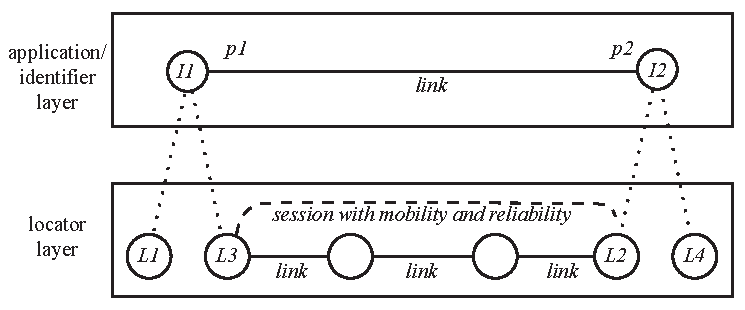
\includegraphics[scale=0.80]{figures/identloc2.pdf}
\caption{A more efficient version of Figure~\ref{fig:identloc}.}
\label{fig:identloc2}
\end{figure}

In the identifier layer, the link between {\it I1} and {\it I2}
is uniquely identified at one end by {\it I1, p1}, where {\it p1}
is a port number, and uniquely identified at the other end by
{\it I2, p2}.
Note that
the identifier layer is more like an application layer than an IP
layer in that it has no forwarding---only direct links between pairs
of communicating endpoints.
Consequently, once the link has been set up, there is absolutely
no need to transmit {\it I1} and {\it I2} in data messages.
Each endpoint simply uses the port number to pass messages unambiguously
across the layer boundary.
Figure~\ref{fig:identloc2} has many similarities with TCP Migrate
\cite{tcp-migrate} and Serval \cite{serval,serval-icnp}, which are other
proposals for SLM.


% This work is licensed under
% http://creativecommon.org/licenses/by/3.0/
\section{Composition of the patterns}
\label{sec:sec7}

\subsection{Structural modeling}
\label{sec:structural}

The geomorphic view of networking is rigorously defined and can
be formalized.
We have formalized various aspects of the geomorphic view in
Alloy, which is the modeling language of the Alloy 
Analyzer \cite{alloy-book},
and in Promela, which is the modeling language of the Spin model
checker \cite{Spin}.
These are {\it structural models}.

Networking researchers and practitioners are accustomed to {\it analytical models},
which are also formal, but quantitative rather than structural.
One can assign numbers to some symbols in an analytical model,
give the numbers and model to a suitable evaluator, and receive
numbers for other symbols in the model.

Structural models are similar, 
except that evaluation is logical rather than quantitative.
We assume that some formulas in a model are true,
give the assumptions and the model to a suitable evaluator such
as the Alloy Analyzer or Spin,
and receive information about the truth of other formulas.
We either learn that a formula is true, or get a counterexample
showing why it is not true.

Sections~\ref{sec:sec3} through \ref{sec:sec6} should have made
clear why the term we use to describe these models is
{\it structural}.
We use them to describe hardware and software structures within
networks,
and to compare mechanisms based on where their structures are
similar and different.
We also use them to show how structural decisions constrain other
decisions and affect important properties such as scalability
and interoperability.
In the next subsection, we will mention some additional knowledge
gained with the help of structural modeling. 

\subsection{Generating the design space of mobility}
\label{sec:design}

An instance of mobility is an isolated
episode in which one layer member changes
its attachment from one underlay member to another.
One of our goals is to give network architects the freedom to handle
any instance of mobility with any mobility pattern at any level of
the layer hierarchy.
This should enhance efficiency and scalability by
allowing solutions that are finely tuned to the characteristics of
the problem they are solving.

The first step was to identify the two possible implementation patterns
and to provide sufficiently abstract versions of them
(Section~\ref{sec:sec3}).
The next step, taken in this section, is to show that any instance of
mobility can be implemented with either pattern at almost any level of
the layer hierarchy.

In the left column of Figure~\ref{fig:lift}, top half, we see a
fundamental instance of mobility in which the old and new locations
are in the same layer at Level 0.
As notated, the channel at Level 1 can be preserved by session-location
mobility (SLM) at Level 0.
In the left column, bottom half, we see a
fundamental instance of mobility in which the old and new locations
are in different layers at Level 0.
As notated, a channel at Level 2 can be preserved by dynamic routing
mobility (DRM) at Level 1.

\begin{figure}
\label{sec:fig:lift}
\centering
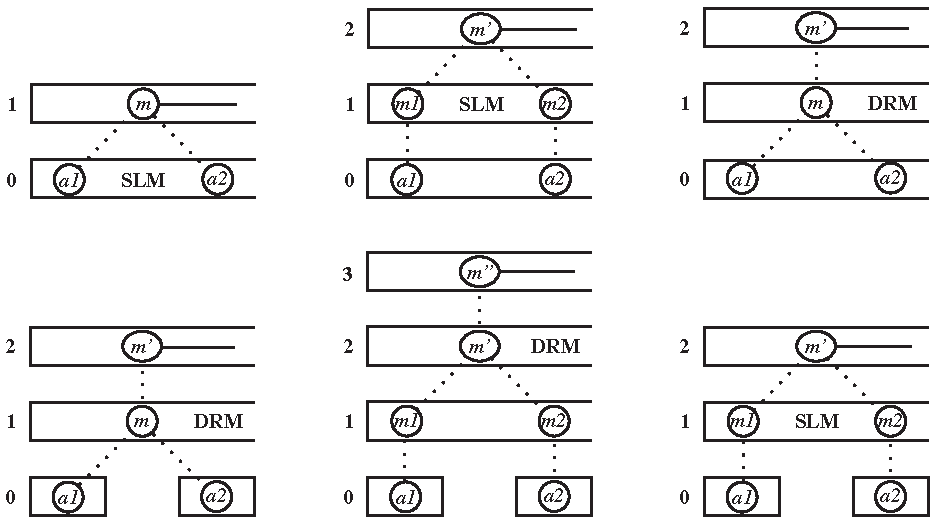
\includegraphics[scale=0.75]{figures/lift.pdf}
\caption{Generating the design space of mobility.}
\label{fig:lift}
\end{figure}

The middle column of the figure shows the effects of a ``lifting''
transformation in which each mobility implementation is moved up a level
in the hierarchy.
The purpose is to show that mobility can be implemented in many different
places, if the current architecture allows it or the designer has
control of the content and design of relevant layers.
In each case member {\it m} at Level 1 is replaced by two members
{\it m1} and {\it m2}.
Neither {\it m1} nor {\it m2} is mobile, as each has a stationary
registration in Level 0 throughout its lifetime.
Now member {\it m'} at Level 2 is mobile.
As shown in the figure (top), a channel in Level 2
with {\it m'} as its higher endpoint
can be preserved by SLM at Level 1. 
Or, as shown at the bottom, a channel in Level 3 with {\it m''} as
its higher endpoint and {\it m'} as its lower endpoint can be preserved
by DRM at Level 2.

The right column of the figure shows where one implementation pattern
can be replaced by the other.
To replace SLM by DRM (top right), it is necessary to lift the channel
up one level.
To replace DRM by SLM (bottom right), the channel can stay at the same
level, but the mobility must be lifted up a level.

Figure~\ref{fig:lift} illustrates the crucial point that mobility
is about name spaces and member identities in individual layers,
and about the mappings between these concepts in adjacent layers.
Identity is a fluid concept in software systems, which is why mobility
is fluid, and can be pushed around an architecture to appear in
different places.

If mobility is fluid, and different implementations are used for
different purposes at different levels of an architecture,
it follows that any layer could include implementations of either or
both mobility patterns.
Is this a problem?
We have proved that it is not, at least for implementations of the
patterns as modeled in Alloy.
Verification with the Alloy Analyzer shows that the two patterns
can be freely composed, in the same layer or
different layers of the same hierarchy.
They will work together without interference or other
undesirable interactions \cite{cnm}.

The limitation of this theoretical result is that,
to benefit from proven
compositionality,
implementations must maintain the minimal separation of concerns
inherent in our model of the geomorphic view.
If real implementations have state dependencies or interfering actions
that are not represented in our model, they are not necessarily
compositional even if the theorem says they are.
In effect the model is presenting sufficient
conditions for compositionality, which can be used as design guidelines
for real systems.

\subsection{Composition in Mobile IPv6}
\label{sec:mipv6}

As we saw in Section~\ref{sec:sec5}, Mobile IPv4 is an instance of DRM.
Mobile IPv6 \cite{mipv6old,mipv6new} uses a similar DRM mechanism, and
also composes it with the SLM mechanism described in 
Section~\ref{sec:sec6}.
We first consider the DRM mechanism.

Figure~\ref{fig:mipv6drm} is the Mobile IPv6 version of 
Figure~\ref{fig:mipv4}.
Note that Mobile IPv6 has no foreign agents, as their functions are
performed by the mobile hosts themselves.
In the figure, both the old attachment of {\it M} at {\it CO1}
and its new attachment at {\it CO2} are shown.
Normal routers are not shown, being replaced by ellipses in the
paths consisting of normal links.

\begin{figure}
\centering
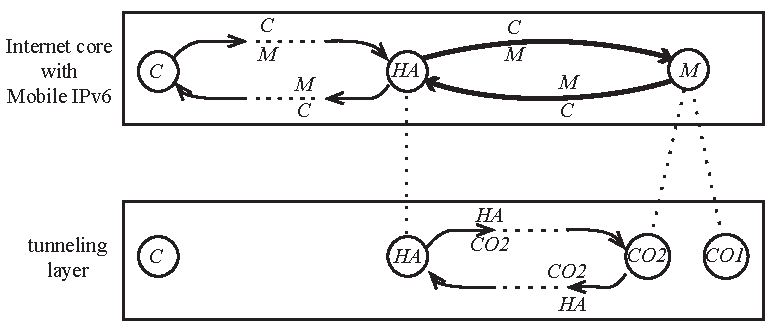
\includegraphics[scale=1.00]{figures/mipv6drm.pdf}
\caption{The paths of messages to and from mobile host {\it M} with
the dynamic-routing mobility mechanism of Mobile IPv6.
Special links are drawn with heavier lines.
Only the links employed in the path are shown.}
\label{fig:mipv6drm}
\end{figure}

Figure~\ref{fig:mipv6drm} also differs from Figure~\ref{fig:mipv4}
in showing the source and destination addresses of the messages on
every link (source on top, destination below).
Thus a message in the core layer with source {\it C} and
destination {\it M} is forwarded on a special link from {\it HA} to
{\it M}.
The implementation of this special link in the tunneling layer 
encapsulates the message in another message with source {\it HA}
and destination {\it CO2}, and sends it through normal IP links and
routers.

Figure~\ref{fig:mipv6drm} also differs from Figure~\ref{fig:mipv4}
in showing the paths of return messages from {\it M} to {\it C}.
In contrast to MIPv4, return messages from {\it M} travel on a
special link as far as {\it HA}.
At {\it HA} they enter the realm of normal links and routers.
There is no problem with ingress filtering because {\it M} belongs to
the address block of {\it HA}'s subnetwork, so {\it M} is a normal
source address at that location. 

The big problem with Mobile IP is the path cost of routing every
message through a mobile host's home agent.
Path cost is even worse in Mobile IPv6 than in Mobile IPv4, because
it is incurred by messages {\it from} a mobile host as well as
messages {\it to} it.
To reduce this problem, Mobile IPv6 standardizes a version of
SLM called ``route optimization,'' as already presented in
Section~\ref{sec:sec6}.
SLM is used only after the session between {\it C} and {\it M}
is established, and only if both endpoints have the protocol capability.

Figure~\ref{fig:mipv6slm} shows the SLM mechanism of Mobile IPv6 in
the same context as its DRM mechanism in Figure~\ref{fig:mipv6drm}.
For simplicity, this figure uses simple encapsulation as in 
\cite{mipv6old}.
After the endpoints have exchanged messages to set up SLM,
they send messages on special links implemented in the tunneling layer.
Note that these are {\it different} special links than those used
by DRM (Figure~\ref{fig:mipv6drm}).
The DRM special links involve {\it HA} and will change when {\it M}
moves.
The SLM special links do not involve {\it HA}, and will not change
from the perspective of the core layer when {\it M} moves.
With SLM, the only role played by {\it HA} in the tunneling layer is to
store the directory entry for {\it M}.
It is not needed originally because when SLM begins the two endpoints
are already connected and know each other's locations in the tunneling
layer, but it may be needed in case of simultaneous handoff.

\begin{figure}
\centering
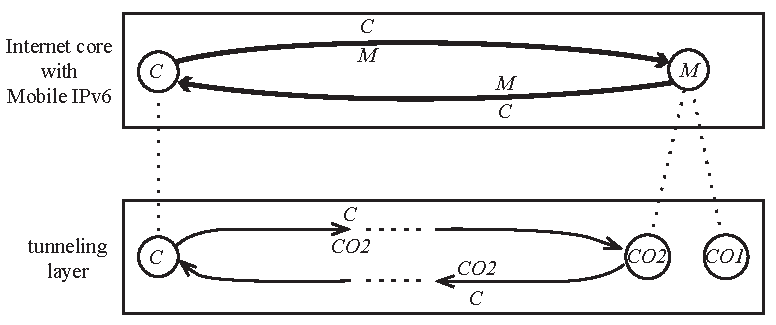
\includegraphics[scale=1.00]{figures/mipv6slm.pdf}
\caption{The paths of messages to and from mobile host {\it M} with
the session-location mobility mechanism of Mobile IPv6.
Special links are drawn with heavier lines.}
\label{fig:mipv6slm}
\end{figure}

Figure~\ref{fig:mipv6slm} also shows the SLM mechanism of Mobile IPv6
in the same context as Figure~\ref{fig:identloc}.
The ``Internet core with Mobile IPv6'' layer in
Figure~\ref{fig:mipv6slm} is the same as the identifier layer in
Figure~\ref{fig:identloc}.
The tunneling layer in
Figure~\ref{fig:mipv6slm} is the same as the locator layer in
Figure~\ref{fig:identloc}.

So far our discussion of the Internet core/identifier
layer has been limited
to its links.
We have seen that {\it C} and {\it M} may have a choice of links
over which to send their messages.
Because the network path associated with each link is different,
its performance may be different.
It is the job of TCP in the Internet core/identifier layer to
smooth over any difficulties caused by diverse paths, for example
by ensuring that messages are delivered to an application layer in
FIFO order.

The design space generated in
Section~\ref{sec:design} is intended primarily for compositions
in which different instances of mobility are managed by different
mechanisms or at different levels of the architecture.
Composition in Mobile IPv6 is a little different because the exact same
instance of mobility---pictured in the figures as {\it M}'s change
of attachment from {\it CO1} to {\it CO2}---is being handled simultaneously
by both forms of mobility.
The DRM implementation is in the core/identifier layer, while the SLM
implementation is in the tunneling/locator layer.
DRM is the default mechanism, because SLM can only be used if both
endpoints are SLM-enabled.


% This work is licensed under
% http://creativecommon.org/licenses/by/3.0/
\section{Design considerations related to mobility}
\label{sec:sec8}

Mobility mechanisms lie close to the heart of networking, so they are
related to many other communication services and aspects of
networking.  In this section, we touch briefly on several other topics
closely related to mobility.

\subsection{Multihoming}
\label{sec:multihoming}

Increasingly, mobile devices connect to the Internet
via multiple interfaces ({\it e.g.,}
a laptop with WiFi and wired Ethernet
interfaces, a smartphone with WiFi and cellular interfaces, or a
virtual machine running on a physical server with multiple wired
Ethernet interfaces).  
Since these interfaces usually connect to
different administrative domains ({\it e.g.,}
a campus WiFi network and a
commercial cellular provider), they must have different IP addresses in
different address blocks.
There is no name for the Internet host itself, and no way to
route to the host itself rather than a specific one of its interfaces.

{\it Sequential multihoming} is the use by a host of multiple
interfaces, one after the other, during the lifetime of a channel.
A mobility mechanism can be used to implement sequential multihoming;
in principle either of the mobility patterns
can be used to provide it.

If we look at the specific real mobility protocols 
in Sections~\ref{sec:sec4} through \ref{sec:sec6}, however,
we see that the DRM protocols in Sections~\ref{sec:sec4} and 
\ref{sec:sec5} work with a single IP address per host, while the
SLM protocols in Section~\ref{sec:sec6} work with multiple IP addresses
per host.
This is an artifact of where these protocols sit in the IP stack rather
than an inherent property of the implementation patterns,
but it does mean that these SLM implementations are currently a better
match for multihoming than these DRM implementations.

{\it Simultaneous multihoming} allows a host to use its multiple
interfaces to contribute bandwidth to the same channel simultaneously.
Simultaneous multihoming
is closely related to sequential multihoming and therefore
to mobility, but not strictly the same because the multiple
interfaces of a host might not be allowed to {\it change} during
the lifetime of a channel.
Of course, what we really want is simultaneous {\it and} sequential
multihoming, which is a
little more complex than sequential multihoming because it requires
protocol extensions so that a layer member can
have and use more than one attachment at a time. 
All of HIP, ILNP, LISP Mobile Node, and Serval
already have session protocols capable of simultaneous multihoming.

Because there is such a close association between host multihoming
and mobility, the well-known multihoming protocols
Multipath TCP~\cite{RFC-6824} 
and the Stream Control Transmission Protocol (SCTP)~\cite{RFC-4960}
are worth studying.
They have been used enough to gather experience on the performance
aspects of switching from one interface to another, and on how performance
affects the buffering and rate control in real transport (session)
protocols such as TCP.
This experience is as relevant to mobility as it is to multihoming.

\subsection{Anycast}

Increasingly, the Internet is a platform for users to
access services hosted on multiple servers in multiple locations.
The appropriate network abstraction for their requirements
is {\it anycast},
in which a service has an {\it anycast name} that corresponds
to a group of servers offering the service.
A request for a communication channel to the service can result in a
channel to any member of the group of servers.

For simple query-response services like DNS,
all server replicas can share a single locator ({\it i.e.,} an IP address),
and rely on IP routing to direct client requests to one of the server
replicas.  
However, IP routing does not guarantee that multiple
messages sent to the same IP address would reach the same server
replica. 
In today's Internet, a domain name
for a geo-replicated service
can map to multiple IP addresses, one for each server replica.
This supports communication services with multiple message exchanges
between client and server.
It is different from mobility, however, because the
higher-level domain name has nothing to do with the channel after
the initial DNS lookup.

Alternatively, anycast could be combined with SLM, as it is in
Serval~\cite{serval,serval-icnp}.
A Serval identifier is an anycast name, and is registered as
located at a dynamic group of servers in the locator layer.
When a request for a channel to an identifier is 
handled by the Serval session protocol,
the protocol selects the locator of some member of the
group.
In contrast to the previous paragraph, the identifier remains
the name of the channel's higher endpoint throughout its lifetime.
The SLM session protocol can thus maintain the channel through both
mobility events and changes to the membership of the server group.

\subsection{Subnetwork mobility}

Mobility proposals typically focus on the
movement of a single mobile endpoint, like a mobile device or a virtual
machine.  However, in some scenarios a subnetwork serving
multiple endpoints can move from one location to another.  
For example, a
fast-moving bus, train, or plane may carry a LAN
that provides network
connectivity to a large collection of passengers.  

Dynamic-routing
mobility in a hierarchical layer
naturally handles subnetwork mobility by updating the routes used
to reach the entire aggregated block of names.
For example, Boeing had an early in-flight WiFi service
that provided seamless mobility for airline passengers by associating
each international flight with an IP address block, and announcing the
block into the global routing system at different locations as the
plane moved~\cite{connexion}.  However, this solution required all
interdomain routers in the Internet to store and update fine-grained
routing information, leading to high overhead.  

In our recent work~\cite{cnm}, we have shown that subnetwork
mobility is merely the mobility of the gateway's attachment to the
larger network, and is implemented with the same two patterns as
mobility of endpoints.
We identified several applications of the design
patterns that seem promising
for handling combinations of subnetwork mobility and endpoint
mobility. 
These solutions have the property that the mechanism for subnetwork
mobility (a bus moves its access point from one roadside LAN to another)
is completely independent of the mechanism for endpoint mobility
(a user with a laptop gets on and off the bus).
Nevertheless, it is not yet clear which solutions for
subnetwork mobility would be most viable in practice.

\subsection{Incremental deployment and interoperation}

Deploying new protocols that span
administrative domains is always challenging, since the Internet
is a federated
infrastructure and cannot easily have everyone upgrade to a new
protocol at the same time.
Most real deployments are DRM mechanisms that
operate within a single administrative domain ({\it e.g.,}
cellular networks, Ethernet LANs, or data-center networks),
or require support only from the mobile endpoint and a small number of
routers ({\it e.g.,} Mobile IPv4).  

It is not surprising that most real mobility implementations use DRM,
because SLM entails many more deployment hurdles.
There can be a new set of identifiers, a new global directory service,
changes to both endpoints, and even
changes to the service interface that are visible to applications.
The early SLM protocol TCP Migrate \cite{tcp-migrate} is probably
the most deployable, requiring only changes to the operating system
at the participating endpoints, but even so it has not had significant
deployment.

Nevertheless, as noted in the introduction,
the pressure for better network mobility support is mounting.
Ubiquitous computing may be a particularly powerful motivator,
because an enormous number of sensors and actuators will require
network access.
This could accelerate the adoption of IPv6, enabling many
other changes in its wake.

For incremental deployment, an SLM-enabled host can interoperate
with a legacy host in a degraded mode in which mobility does not work
but other functions do.
For full mobility, an SLM-enabled host can interoperate with
a legacy host through a proxy or other middlebox.
This raises many new questions concerning how a middlebox is
introduced into the path between the hosts, and on the scalability
of stateful middleboxes.
These new questions must be added to the perennial list of old
interoperability questions, such as how to traverse
NAT boxes.
Identifying
effective ways to deploy these protocols incrementally remains an
active area of research and standards work.

\subsection{Security}

All mobility solutions raise important questions about
security.  
In DRM, who is authorized to announce
routing changes for an address or address block?  
In SLM, who is authorized to update the directory service and a
mobile endpoint's correspondents?  
Answering these questions
successfully requires unforgeable notions of identity, and secure
protocols for sending update messages to routers, directory servers,
and endpoints.  
Can accidental misconfigurations or malicious attacks
overload the routers, directory servers, or endpoints?  Preventing
denial-of-service attacks requires effective ways to limit the work
performed before recognizing that messages are unauthorized.  

As
mentioned in Section~\ref{sec:majordifferences}, some people believe that
SLM protocols face greater security challenges
because arbitrary endpoints can initiate updates to global layer state.
On the other hand, SLM protocols provide for persistent identifiers
which can be used as the basis for authentication of hosts, a valuable
assistance to security.
SLM protocols that use DNS as the directory
service can update DNS
records with an existing secure protocol~\cite{RFC-2137}.  
Some protocols, like HIP and Serval, embed
an endpoint's public key (or a hash of the key) in the identifier; 
these identifiers support secure communication as well as
authentication.
Still, security is a rich and
important topic warranting a much deeper treatment, especially since
new protocols can easily introduce unforeseen vulnerabilities and new
threats.


% This work is licensed under
% http://creativecommon.org/licenses/by/3.0/
\section{Conclusion}
\label{sec:sec9}

In this chapter we have presented an abstract framework for describing, 
understanding, and comparing approaches to network mobility.  
As illustrations, we have covered several mobility protocols 
in some detail.
We believe the geomorphic model provides a clear and precise way to understand the considerable similarities between different mobility proposals,
allowing discussions to focus on their meaningful distinctions rather than artificial differences in terminology.

We have compared mobility proposals on both qualitative
(deployment constraints, security) and quantitative (resource costs,
latency) criteria.
The basis for making comparisons has been completely {\it structural},
in the sense of {\it structural modeling} as defined in 
Section~\ref{sec:structural}.
This is important because structural comparisons are vastly easier
to obtain than comparisons based on simulation, and should always
be the first step in any evaluation project.

In the interest of brevity, our discussions of quantitative
criteria have merely suggested trends and trade-offs, rather than
providing a more substantive analysis.
A true understanding of metrics such as
storage cost, update cost, and path cost requires a more 
detailed characterization of the proposals, including
supporting technologies such as routing protocols and directory services. 
Scalability depends on how these costs grow as the size of a network
grows within the expected range.
 
Equally important, different mobility mechanisms can be composed.
Even today it would not be surprising to see
dynamic-routing mobility used 
within an administrative domain, while
session-location mobility is used simultaneously
across administrative boundaries.
The ultimate goal would be to compose performance models along with
the mechanisms they are modeling, so that the performance of
a composed solution could be derived from the performance of its
components.   

Today, many Internet applications that could benefit from mobility
use work-arounds instead, satisfying the need for session continuity
with {\it ad hoc} application-specific mechanisms, or simply doing
without \cite{handley}.
This is both an effect and a cause of scant deployment of mobility
mechanisms.
Most existing mobility protocols operate at fairly low levels
in a network architecture, 
specifically the link, network, and transport levels
of the classic Internet stack.
At these levels they are expensive, difficult to deploy, or both.

Many of these limitations are unnecessary, as
the essence of mobility is simply a dynamic binding of more abstract
names to more concrete names.  
As such, mobility can be easily implemented in middleware as a service to
even higher-level application layers.  
We believe that this is a fruitful avenue for further exploration,
particularly because it might be easier to optimize narrowly-targeted
implementations of mobility.

More generally, we believe that the geomorphic view promotes
common terminology, modularity,
separation of concerns, discovery of design patterns,
composition,
rigorous reasoning,
and code reuse in networking.
While widely appreciated by software engineers, 
these concepts have been less central to the study of networking.  
We believe that the geomorphic view should be extended to understand
other important aspects of networking.
We also believe that an appreciation of these concepts would be 
valuable for networking researchers and practitioners alike, 
far beyond the treatment of any one subject like network mobility.


\bibliographystyle{IEEEtran}
\bibliography{ebook}

\end{document}
